\chapter{Benchmark Models and Reference Results}
\label{chap:benchmarks}

%%%%%%%%%%%%%%%%%%%%%%%%%%%%%%%%%%%%%%%%%%%%%%%%%%%%%%%%%%%%%%%%%%%%%%%%%%%%%%%
\section{Motivation}
\label{sec:chap7-motivate}

This thesis is motivated by the desire to obtain Monte Carlo-quality solutions with computationally efficient deterministic neutron transport methods. In particular, this work evaluates the use of \ac{MC} for reactor agnostic \ac{MGXS} generation for high-fidelity neutron transport simulations. The analysis in Part III was dedicated to the evaluation of approximation errors in \ac{MGXS} and multi-group transport methods which appear in the modeling of even simple heterogeneous benchmarks such as a 2D fuel pin cell. The chapters in Part IV develop a new approach based upon statistical clustering to capture spatial self-shielding effects which occur only in large, complex heterogeneous geometries. This chapter presents several heterogeneous \ac{PWR} benchmark models which are used to evaluate the efficacy of the new methodology for \ac{MGXS} generation throughout the subsequent chapters in Part IV.

Each of the heterogeneous benchmarks presented here is derived from the Benchmark for Evaluation And Validation of Reactor Simulations (BEAVRS) \ac{PWR} model~\cite{horelik2013beavrs}. A series of six heterogeous benchmarks were designed to introduce increasingly complex heterogeous features -- and corresponding spatial self-shielding effects -- to the models in order to understand their implications for accurate pin-wise \ac{MGXS} generation. The impact of \acp{CRGT}, fuel enrichment, \acp{BP}, inter-assembly currents, water reflectors, steel baffles and the core barrel and vessel is considered. This chapter details the geometric and material specifications for the individual fuel assemblies, multiple assembly colorsets, and full \ac{BEAVRS} core modeled with different \ac{MGXS} generation schemes throughout Part IV.

In addition, this chapter presents the reference results for each of the six geometries used to evaluate the accuracy of \ac{MGXS} generation with statistical clustering. Since this thesis aims to enable \ac{MC} accuracy in deterministic transport simulations, OpenMC was used to generate the reference results for each of the six benchmarks. This chapter quantifies the source convergence rate for each of the benchmark models using Shannon entropy. In addition, a series of OpenMC simulations were used to calculate reference results for the following three metrics for validation of \ac{MGXS} in OpenMOC:

\begin{itemize}[noitemsep,topsep=0pt]
  \item \textbf{Eigenvalues}
  \item \textbf{Pin-wise fission rates}
  \item \textbf{Pin-wise U-238 capture rates}
\end{itemize}

\noindent The reference results for each of these three metrics were computed with highly converged OpenMC simulations. It is important to recall from Sec.~\ref{sec:chap1-objectives} that this thesis aimed to generate \ac{MGXS} with \ac{MC} in significantly less time\footnote{In this case, ``time'' is synonymous with the number of particle histories simulated with \ac{MC}.} than would be required to generate reference solutions with \ac{MC}. The methodology developed in Part IV aims to make this possible with statistical clustering of ``noisy'' \ac{MC} tallies for \ac{MGXS} generation.

This chapter outlines the geometric and isotopic specifications for each of the six benchmark models in Sec.~\ref{sec:chap7-benchmarks}. The reference results computed with OpenMC for each of the benchmark models are presented in Sec.~\ref{sec:chap7-ref-results}.


%%%%%%%%%%%%%%%%%%%%%%%%%%%%%%%%%%%%%%%%%%%%%%%%%%%%%%%%%%%%%%%%%%%%%%%%%%%%%%%
\section{Benchmark Configurations}
\label{sec:chap7-benchmarks}

The heterogeneous benchmarks modeled throughout Part IV were based on upon the \ac{BEAVRS} \ac{PWR} model~\cite{horelik2013beavrs}. The \ac{BEAVRS} model is a highly-detailed \ac{PWR} specification which was created to validate high-fidelity core analysis methods. Five of the six benchmark models are based upon sub-components (\textit{e.g.}, fuel assemblies) of the full core \ac{BEAVRS} model, while the sixth benchmark is of the full \ac{BEAVRS} core model. Although \ac{BEAVRS} is an axially heterogeneous 3D core model, each of the benchmarks were fabricated in 2D due to the geometric constraints in OpenMOC. In particular, the 2D radial heterogeneity in each benchmark is taken from the axial mid-plane of the \ac{BEAVRS} model. The geometries used two planar surfaces perpendicular to the $z$-axis with reflective \acp{BC} to model the benchmarks as infinitely long in the axial direction (\textit{e.g.}, each benchmark was treated as infinitely homogeneous along the $z$-axis).

%first paragraph: refer to the \ac{BEAVRS} model~\cite{horelik2013beavrs}
%-\ac{BEAVRS} consists of fuel assemblies with four different enrichments and various
%  -sliced to encompass the spacer grid
%    -designed model to stress the geometric modeling capabilities of OpenMC/MOC/CG
%    -grid spacers main axial heterogeneities that induce spatial self-shielding in \ac{LWR}s
%    -stress geometric modeling capabilities since framework developed to eventually support 3D \ac{MOC}
%-HZP

The materials and isotopic compositions in each of the benchmarks are detailed in Sec.~\ref{subsec:chap7-materials}, while the geometric specifications for each pin cell type -- fuel pin, instrument tube, \ac{CRGT} and \ac{BP} -- are tabulated in Sec.~\ref{subsec:chap7-pin-cells}. The first three benchmarks were based upon individual \ac{BEAVRS} fuel assemblies with different fuel enrichments and \ac{CRGT} and \ac{BP} locations as discussed in Sec.~\ref{subsec:chap7-fuel-assms}. The geometric configuration of 2$\times$2 fuel assembly colorsets with and without a water reflector are highlighted in Sec.~\ref{subsec:chap7-2x2-colorsets}. Finally, the key parameters for the full 2D \ac{BEAVRS} core model are presented in Sec.~\ref{subsec:chap7-full-core}.


%%%%%%%%%%%%%%%%%%%%%%%%%%%%
\subsection{Materials}
\label{subsec:chap7-materials}

The models described in this section were comprised of materials from the \ac{BEAVRS} model. The six benchmarks were comprised of some or all of the following materials:

\begin{itemize}[noitemsep,topsep=0pt]
  \item 1.6\% and 3.1\% enriched UO$_2$ fuel
  \item Borated water\footnote{The water consisted of 975 parts per million (ppm) boron.}
  \item Zircaloy 4
  \item Borosilicate glass
  \item Stainless steel (SS304)
\end{itemize}

\noindent The densities and isotopic compositions for each material are detailed in the \ac{BEAVRS} specifications~\cite{horelik2013beavrs} and are reproduced in App.~\ref{app:beavrs-isotopes}. Each of the materials was modeled with cross sections at the temperatures for hot zero power (HZP) conditions.

%%%%%%%%%%%%%%%%%%%%%%%%%%%%
\subsection{Pin Cells}
\label{subsec:chap7-pin-cells}

Each of the six benchmarks were composed of four different types of pin cells -- fuel pins, instrument tubes, control rod guide tubes and burnable poisons. Each of the four pin cell types is displayed in Fig.~\ref{fig:chap7-pin-cells}. The different material types are indicated with different colors. The fuel pin in Fig.~\ref{fig:chap7-pin-1.6} contains UO$_2$ fuel, helium gap and zircaloy cladding. The \ac{CRGT} in Fig.~\ref{fig:chap7-pin-crgt} is modeled in the control rod out configuration from above the dashpot and includes borated water surrounded by zircaloy cladding. The instrument tube in Fig.~\ref{fig:chap7-instr-tube} is filled with air surrounded by two tubes of zircaloy cladding. The \ac{BP} in Fig.~\ref{fig:chap7-bp} geometry is the geometry from above the dashpot in the \ac{BEAVRS} model and consists of eight layers of air, steel, borosilicate glass and zircaloy. Each pin cell is surrounded by borated water which serves as the neutron moderator and coolant. 

The gray borders illustrated in Fig.~\ref{fig:chap7-pin-cells} represent the egg-crate grid spacer structure wrapped around each fuel pin. Each of the six benchmarks was sliced about the $z$-axis in order to encapsulate the fuel assembly grid spacer located at $203.558 \le z \le 209.273$ in the \ac{BEAVRS} model. Next-generation high-fidelity transport methods for reactor analysis must account for the axially-oriented spatial self-shielding effects induced by grid spacers in \ac{LWR} core geometries. Although axial spatial self-shielding effects were not modeled in this thesis, the grid spacers were included in the 2D benchmarks to stress the geometric modeling capabilities recently introduced in OpenMOC to support 3D \ac{MOC} calculations. Future work may build upon the analysis in this thesis to develop \ac{MGXS} generation schemes which account for spatial self-shielding effects from axial heterogeneities such as spacer grids.

\begin{figure}[h!]
\centering
\begin{subfigure}{.5\textwidth}
  \centering
  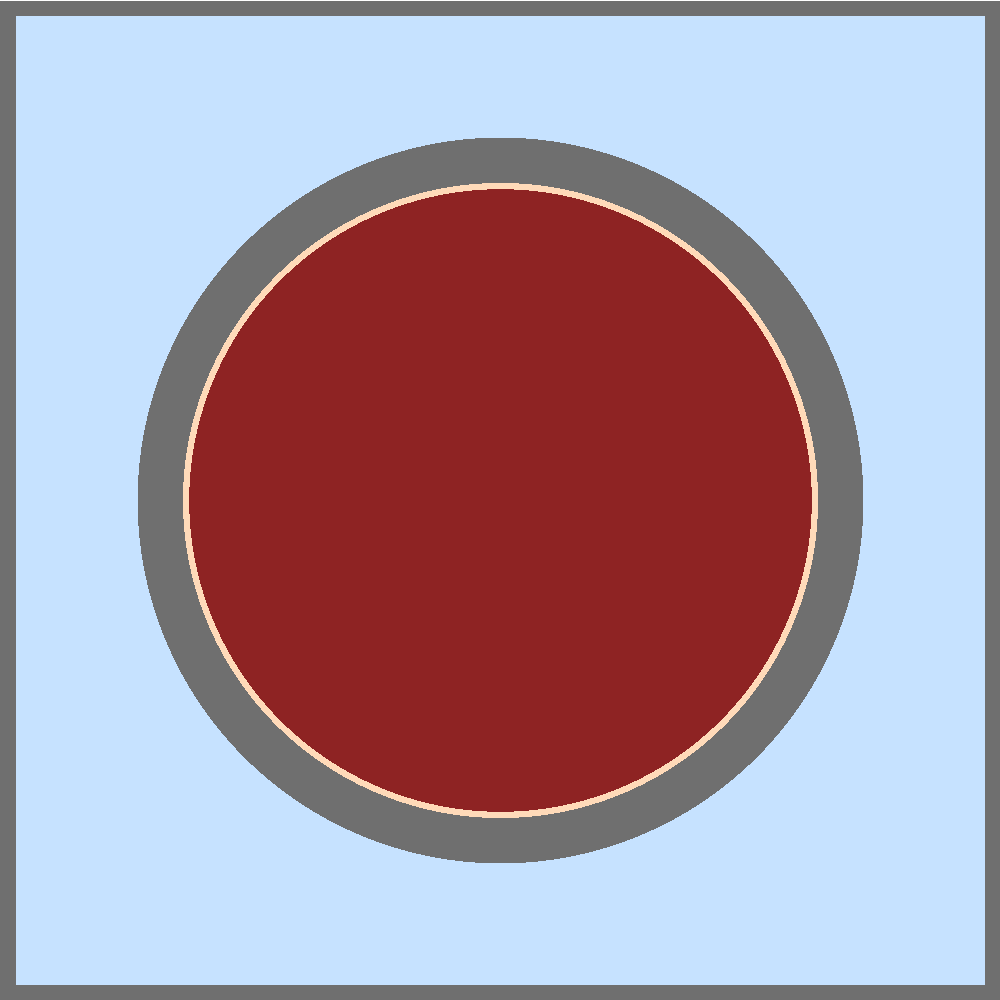
\includegraphics[width=0.9\linewidth]{figures/benchmarks/fuel-pin-16}
  \caption{}
  \label{fig:chap7-pin-1.6}
\end{subfigure}%
\begin{subfigure}{.5\textwidth}
  \centering
  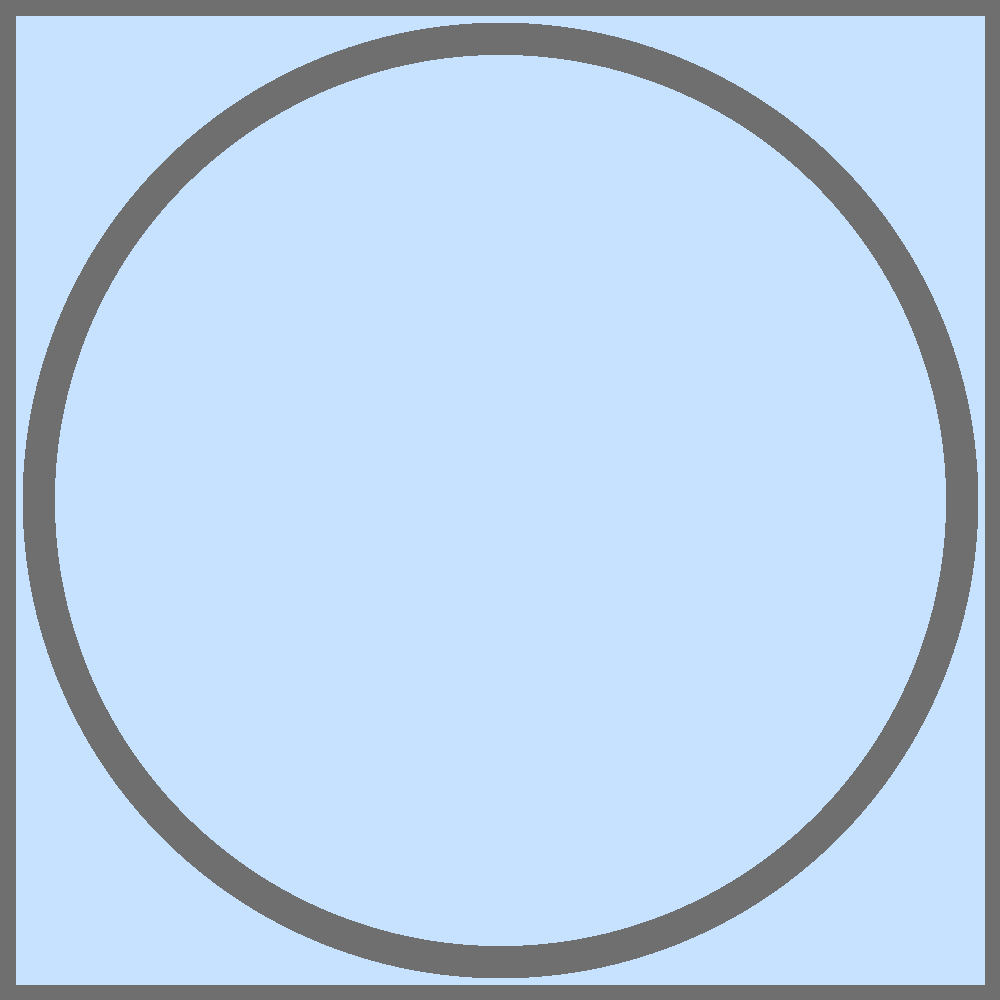
\includegraphics[width=0.9\linewidth]{figures/benchmarks/guide-tube}
  \caption{}
  \label{fig:chap7-pin-crgt}
\end{subfigure}
\begin{subfigure}{.5\textwidth}
  \centering
  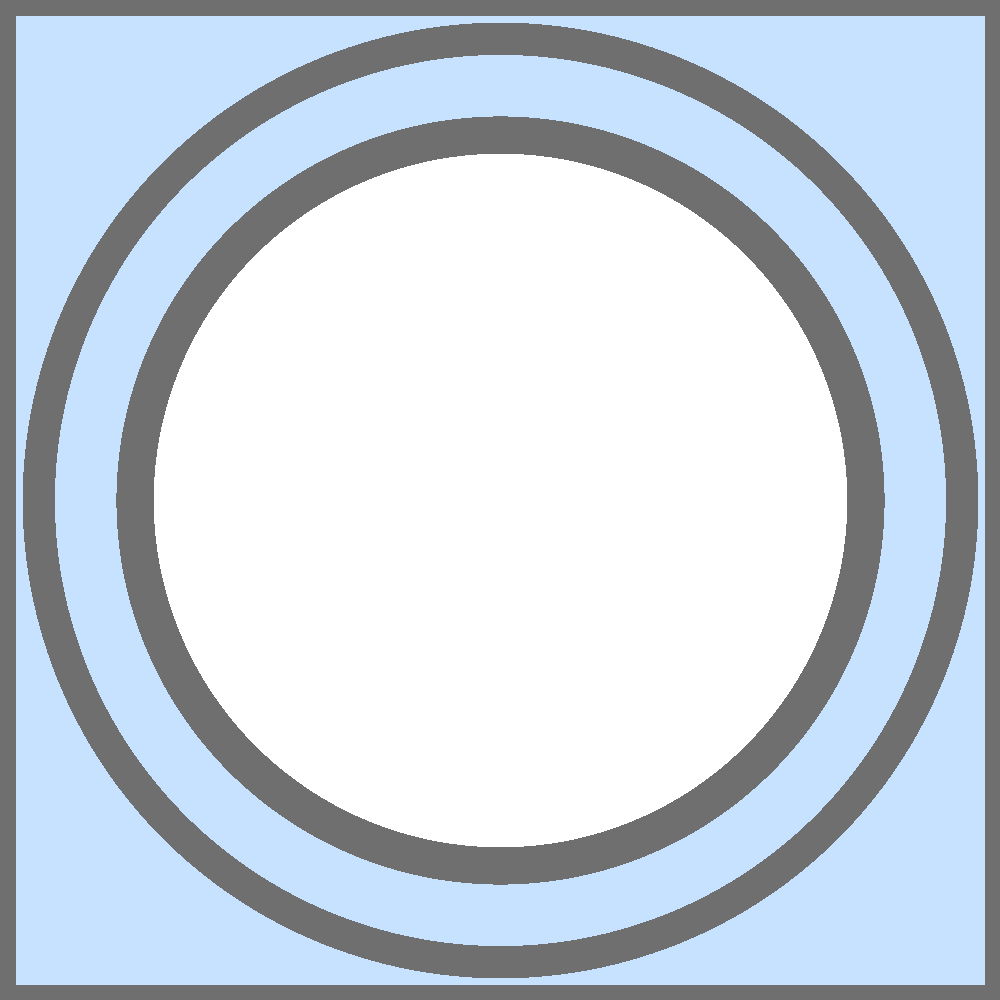
\includegraphics[width=0.9\linewidth]{figures/benchmarks/instr-tube}
  \caption{}
  \label{fig:chap7-instr-tube}
\end{subfigure}%
\begin{subfigure}{.5\textwidth}
  \centering
  
\includegraphics[width=0.9\linewidth]{figures/benchmarks/burn-abs}
  \caption{}
  \label{fig:chap7-bp}
\end{subfigure}%
\caption[BEAVRS pin cell geometries]{1.6\% enriched fuel pin (a), control rod guide tube (b), instrument tube (c) and burnable poison (d). Light blue is borated water, red is UO$_2$ fuel, gray is zircaloy, brown is helium, white is air, green is borosolicate glass, and black is stainless steel.}
\label{fig:chap7-pin-cells}
\end{figure}

The radii for each material zone in the pin cells are detailed in Tab.~\ref{table:chap7-pin-cell-radii}. Each pin is surrounded by borated water and a zircaloy egg-crate grid spacer.  The pin cell pitch is 1.25984 cm and the thickness of the grid spacer is 0.02014 cm.

\renewcommand{\arraystretch}{0.9}
\begin{table}[h!]
  \centering
  \caption[BEAVRS pin cell radii]{Pin cell radii for the \ac{BEAVRS} model.}
  \small
  \label{table:chap7-pin-cell-radii} 
  \vspace{6pt}
  \begin{tabular}{l c}
  \toprule
  \rowcolor{lightgray}
  \multicolumn{1}{c}{\bf Material} &
  \multicolumn{1}{c}{\bf Radius [cm]} \\
  \midrule
  \multicolumn{2}{c}{\bf Fuel Pin} \\
  \midrule
  Fuel &  0.39218 \\
  Helium & 0.40005 \\
  Zircaloy & 0.45720 \\
  \midrule
  \multicolumn{2}{c}{\bf Control Rod Guide Tube} \\
  \midrule
  Borated Water & 0.56134 \\
  Zircaloy & 0.60198 \\
  \midrule
  \multicolumn{2}{c}{\bf Instrument Tube} \\
  \midrule
  Air & 0.43688 \\
  Zircaloy & 0.48387 \\
  Borated Water & 0.56134 \\
  Zircaloy & 0.60198 \\
  \midrule
  \multicolumn{2}{c}{\bf Burnable Poison} \\
  \midrule
  Air & 0.21400 \\
  Stainless Steel & 0.23051 \\
  Air & 0.24130 \\
  Borosilicate Glass & 0.42672 \\
  Air & 0.43688 \\
  Stainless Steel & 0.48387 \\
  Borated Water & 0.56134 \\
  Zircaloy & 0.60198 \\
  \bottomrule
\end{tabular}
\end{table}

%\addtocounter{footnote}{-2}
%\stepcounter{footnote}\footnotetext{The control rod guide tube geometry above the dashpot.}
%\stepcounter{footnote}\footnotetext{The burnable poison geometry above the dashpot.}


%%%%%%%%%%%%%%%%%%%%%%%%%%%%
\subsection{Fuel Assemblies}
\label{subsec:chap7-fuel-assms}

The first three benchmark models are based upon 2D models of individual fuel assemblies extracted from the full core \ac{BEAVRS} model. Each assembly consists of a 17$\times$17 rectilinear array of pin cells in a lattice with a height and width of 21.41728 cm. The stainless steel grid sleeve and water separating each fuel assembly in the full core \ac{BEAVRS} model are not included in the individual models of each fuel assembly. The intra-pin egg-crate grid spacer is included in each benchmark model. The assemblies are modeled with reflective \acp{BC} to simulate an infinite lattice of fuel pins, control rod guide tubes, burnable poisons and instrument tubes. 

\begin{figure}[h!]
  \centering
  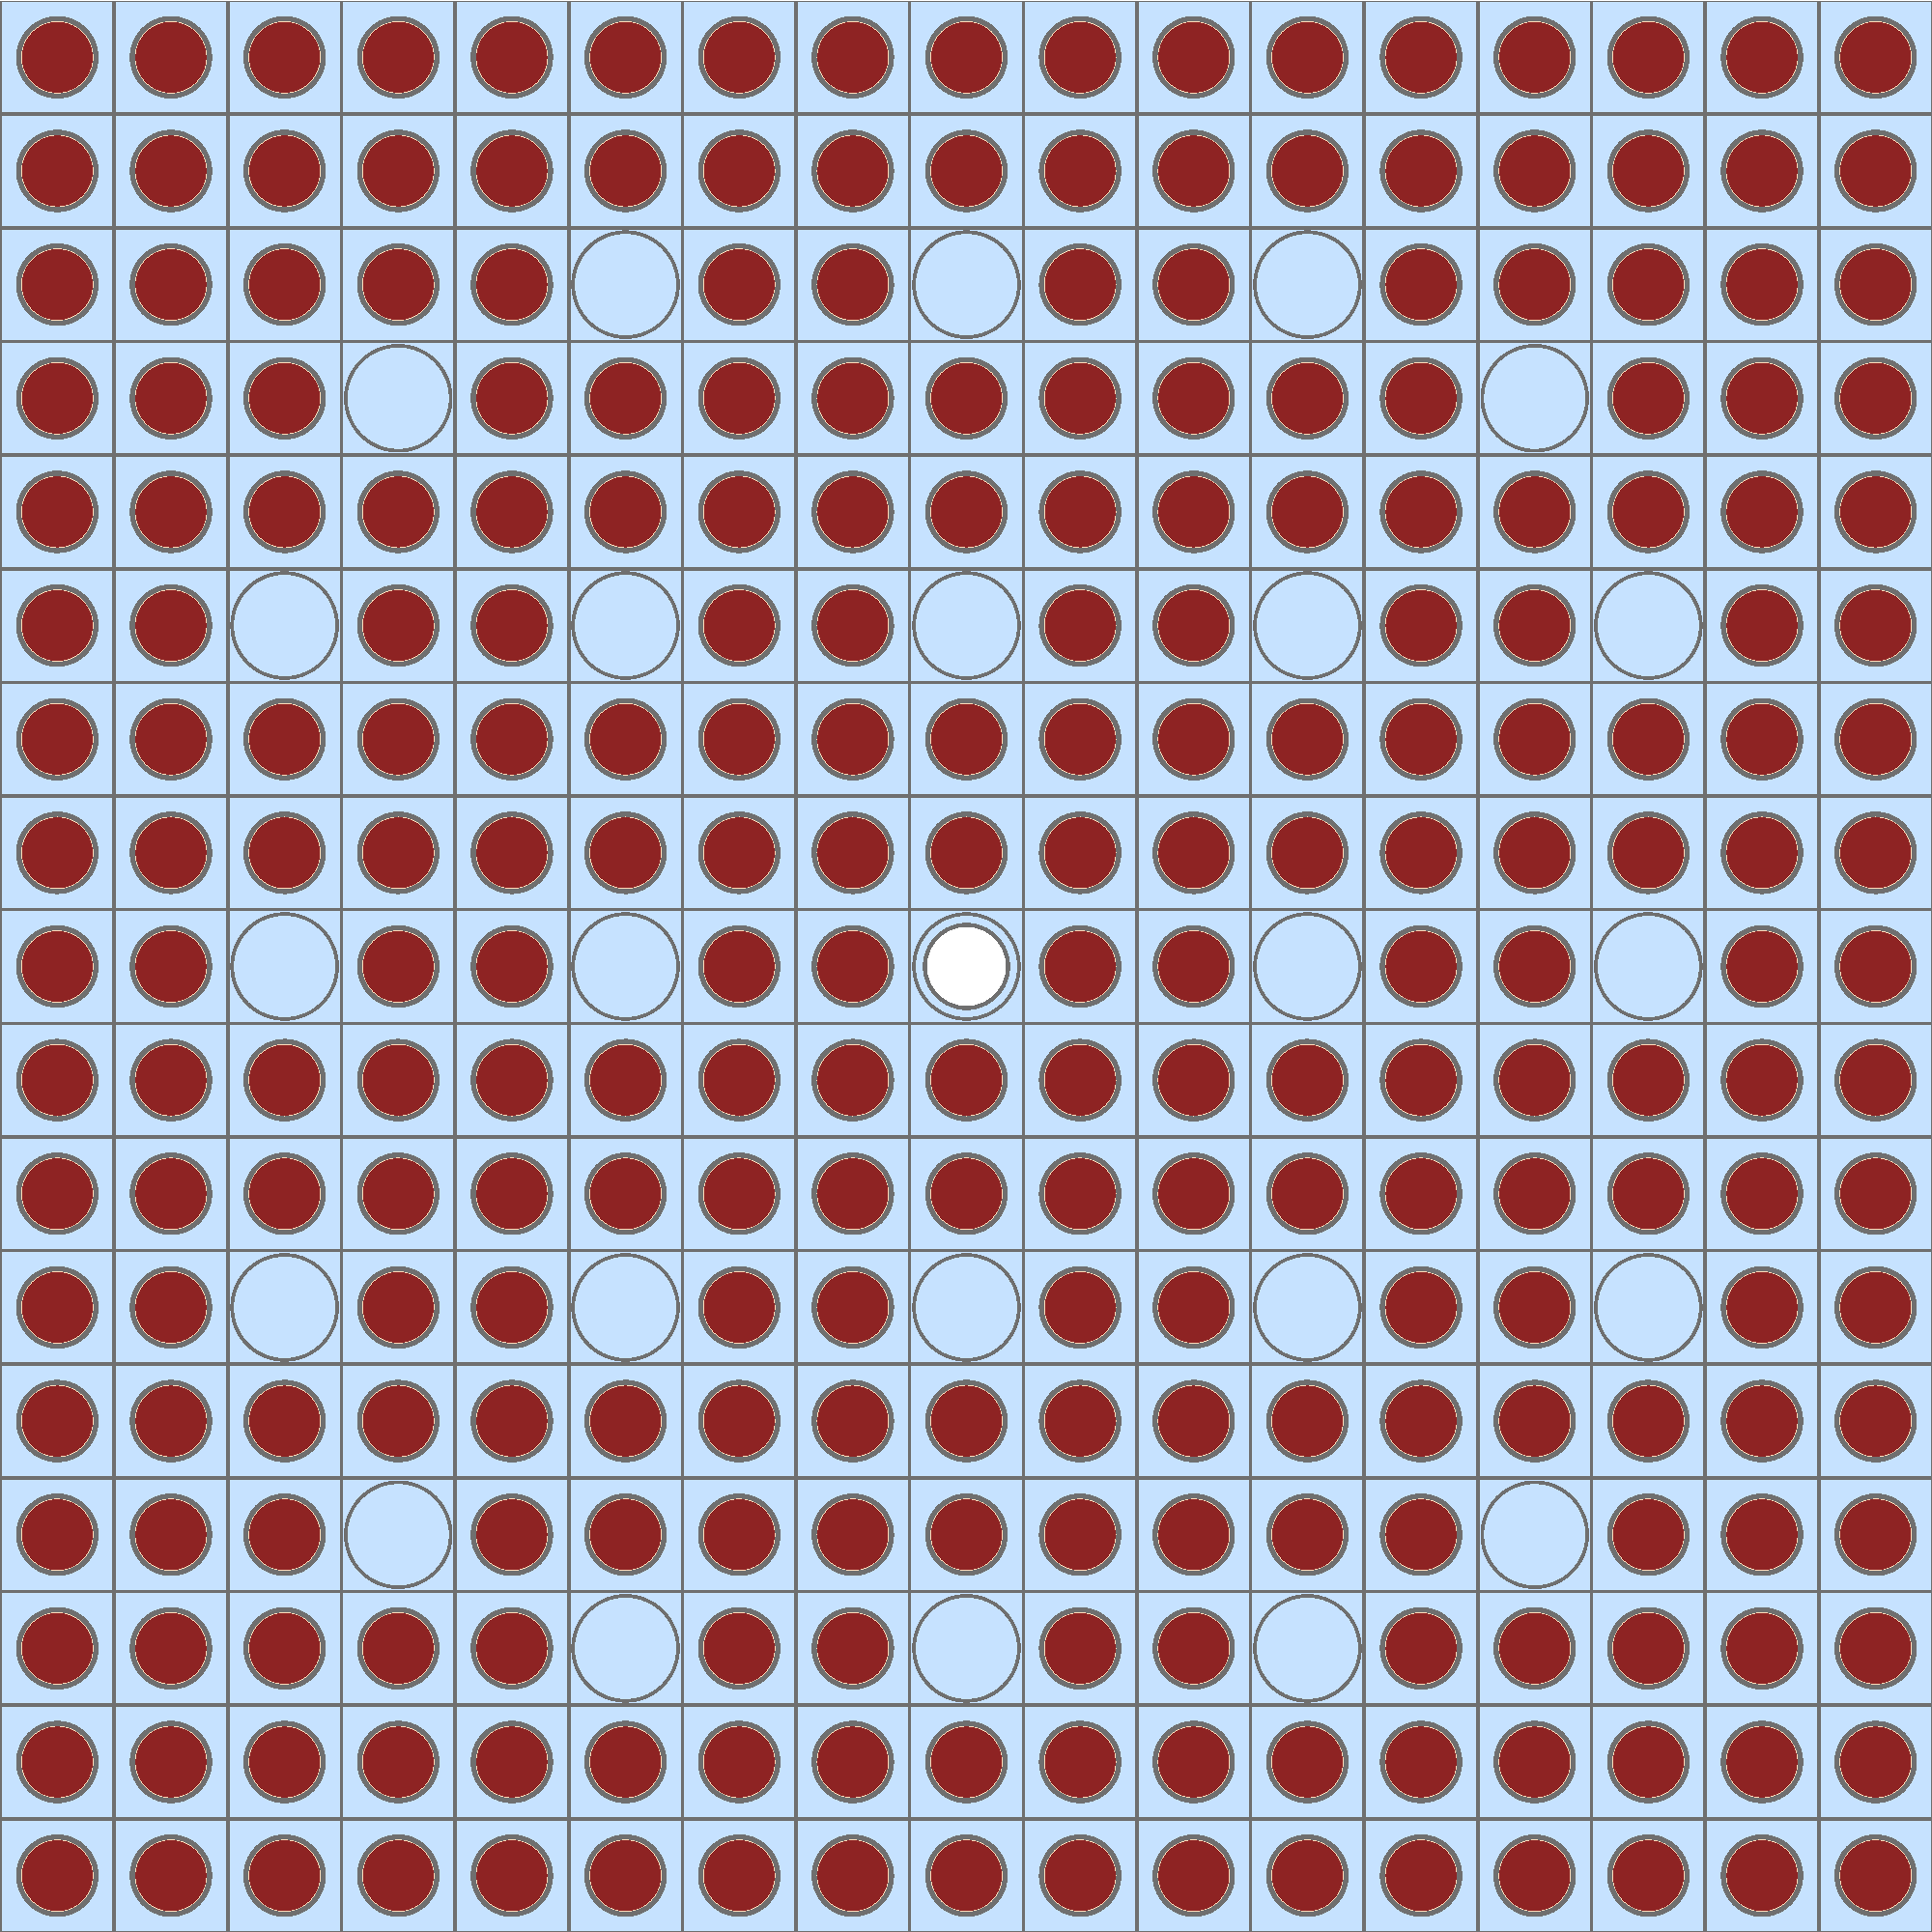
\includegraphics[width=0.65\linewidth]{figures/benchmarks/assembly-16}
\vspace{2mm}
\caption[BEAVRS 1.6\% enriched assembly]{A 1.6\% enriched UO$_2$ fuel assembly without \acp{BP}.}
\label{fig:chap7-assm-16}
\end{figure}

\begin{figure}[h!]
  \centering
  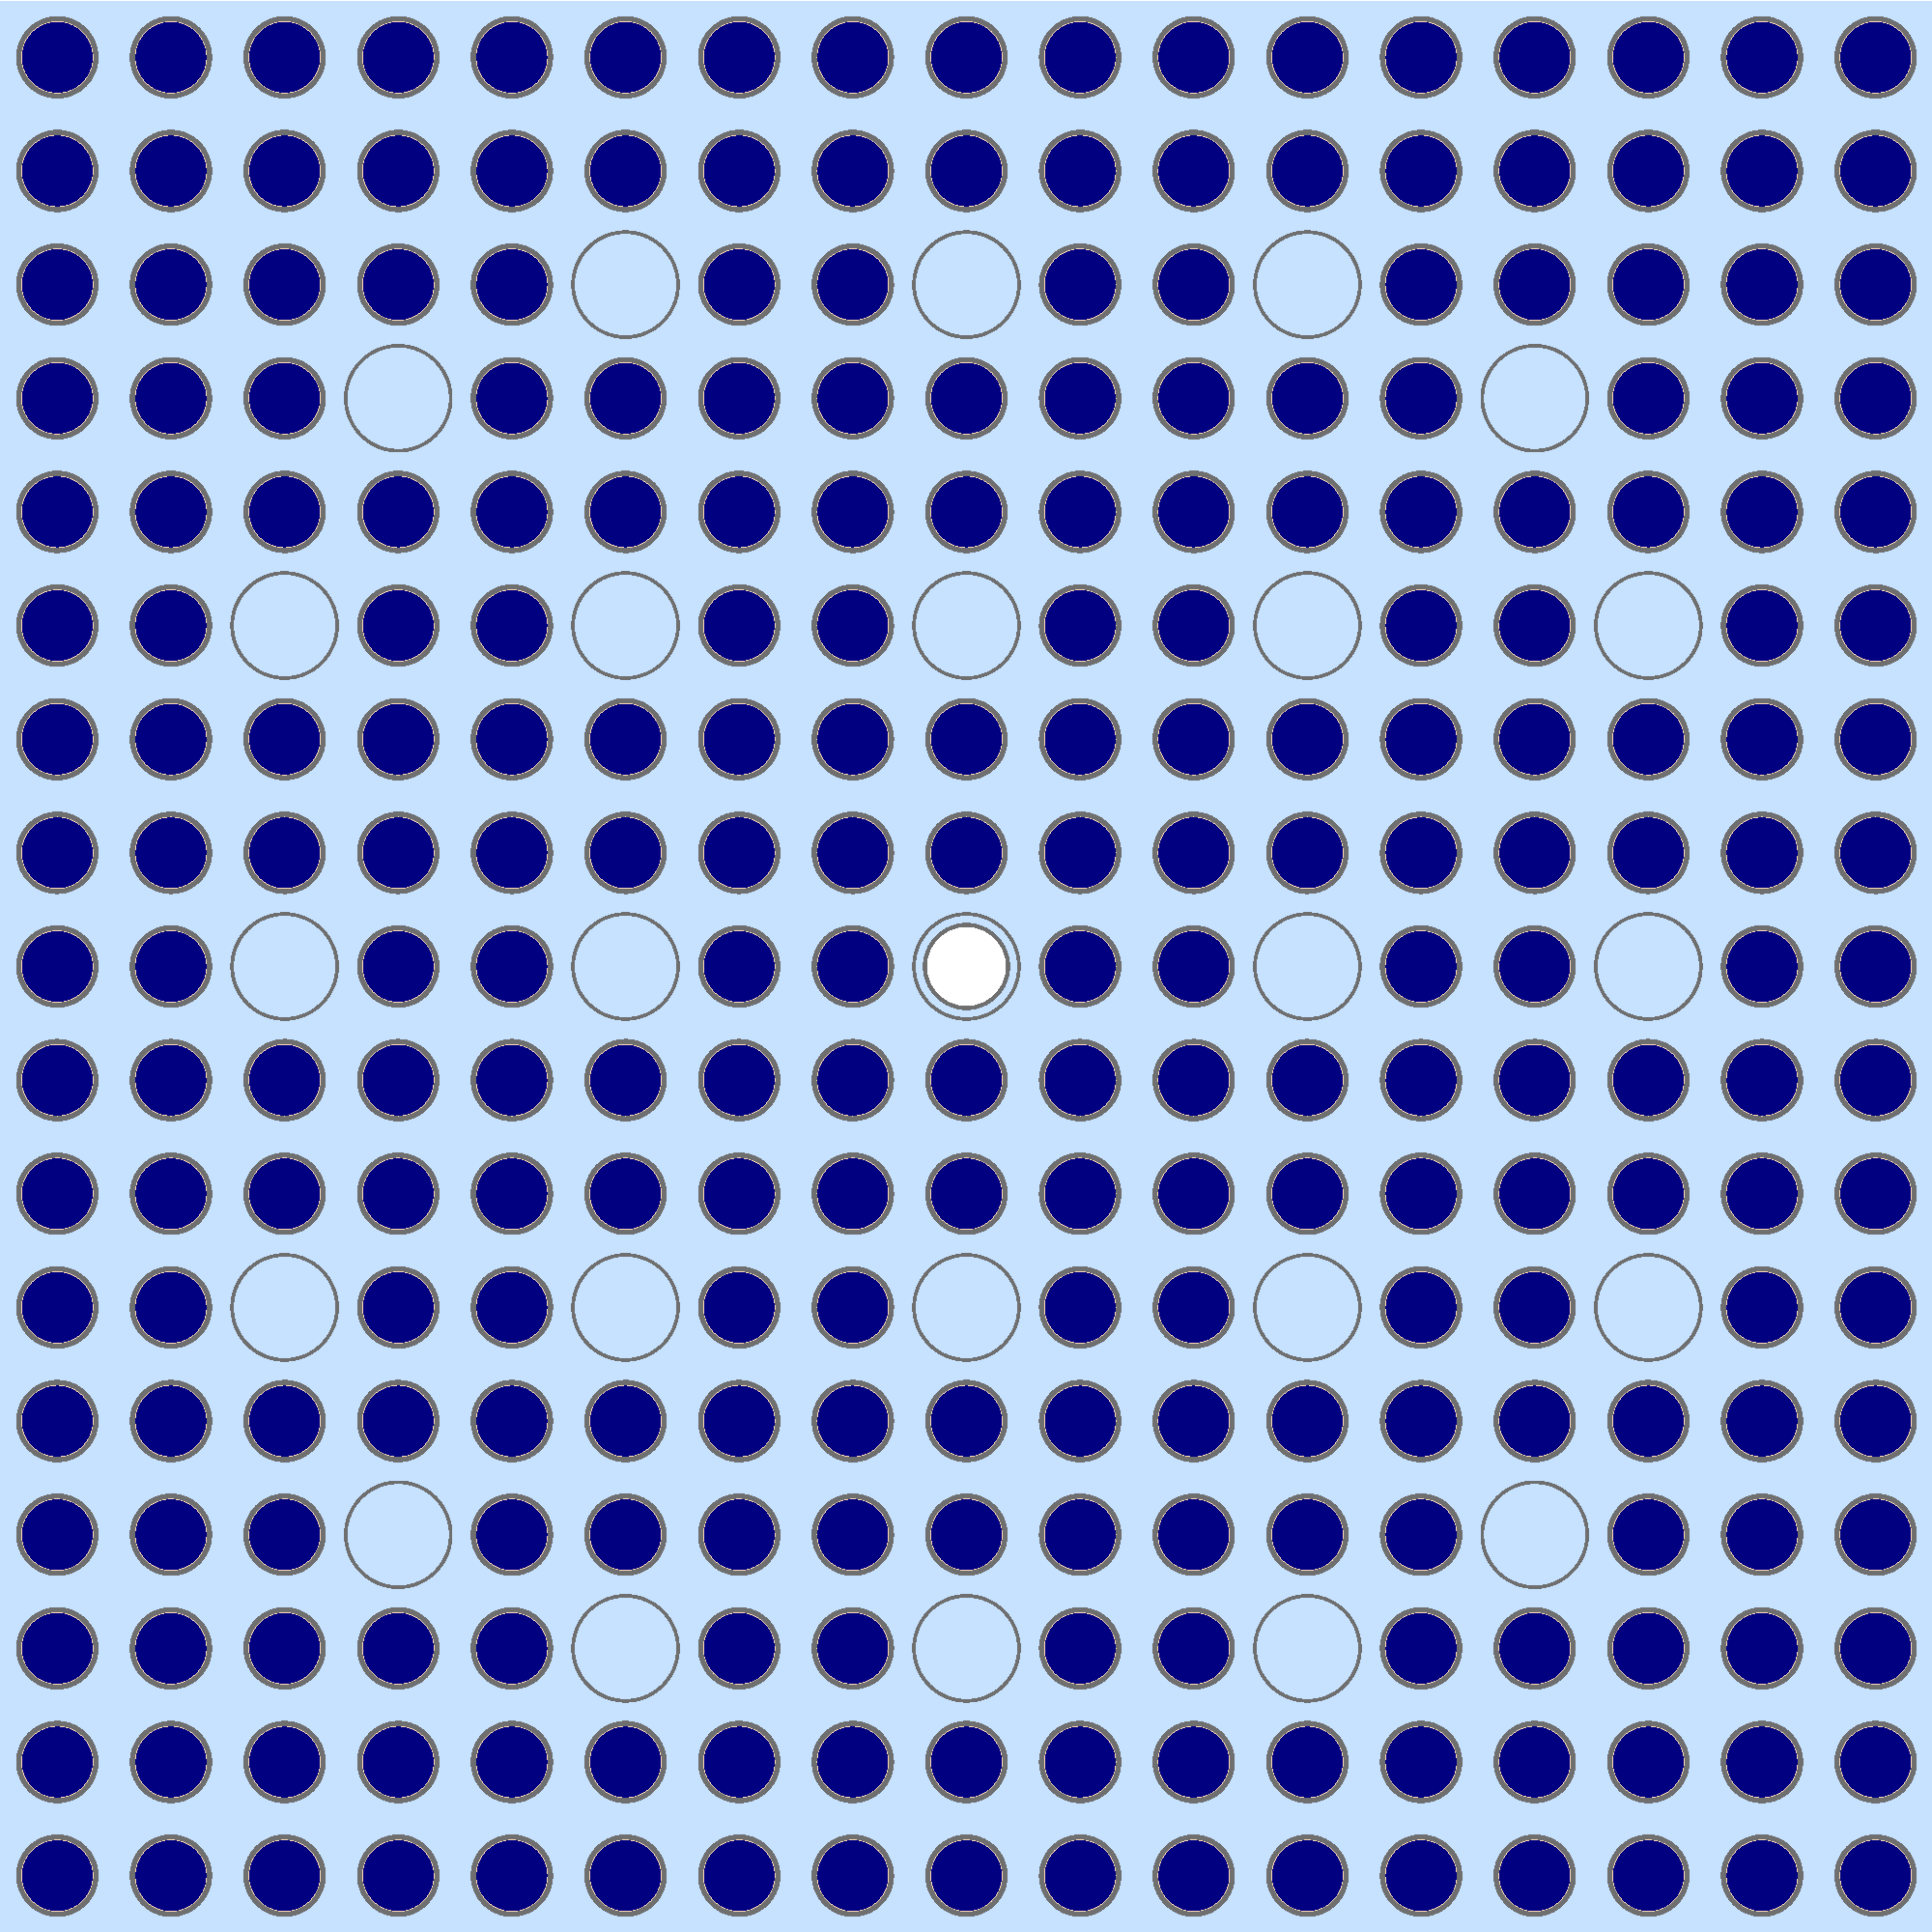
\includegraphics[width=0.65\linewidth]{figures/benchmarks/assembly-31}
\vspace{2mm}
\caption[BEAVRS 3.1\% enriched assembly]{A 3.1\% enriched UO$_2$ fuel assembly without \acp{BP}.}
\label{fig:chap7-assm-31}
\end{figure}

\begin{figure}[h!]
  \centering
  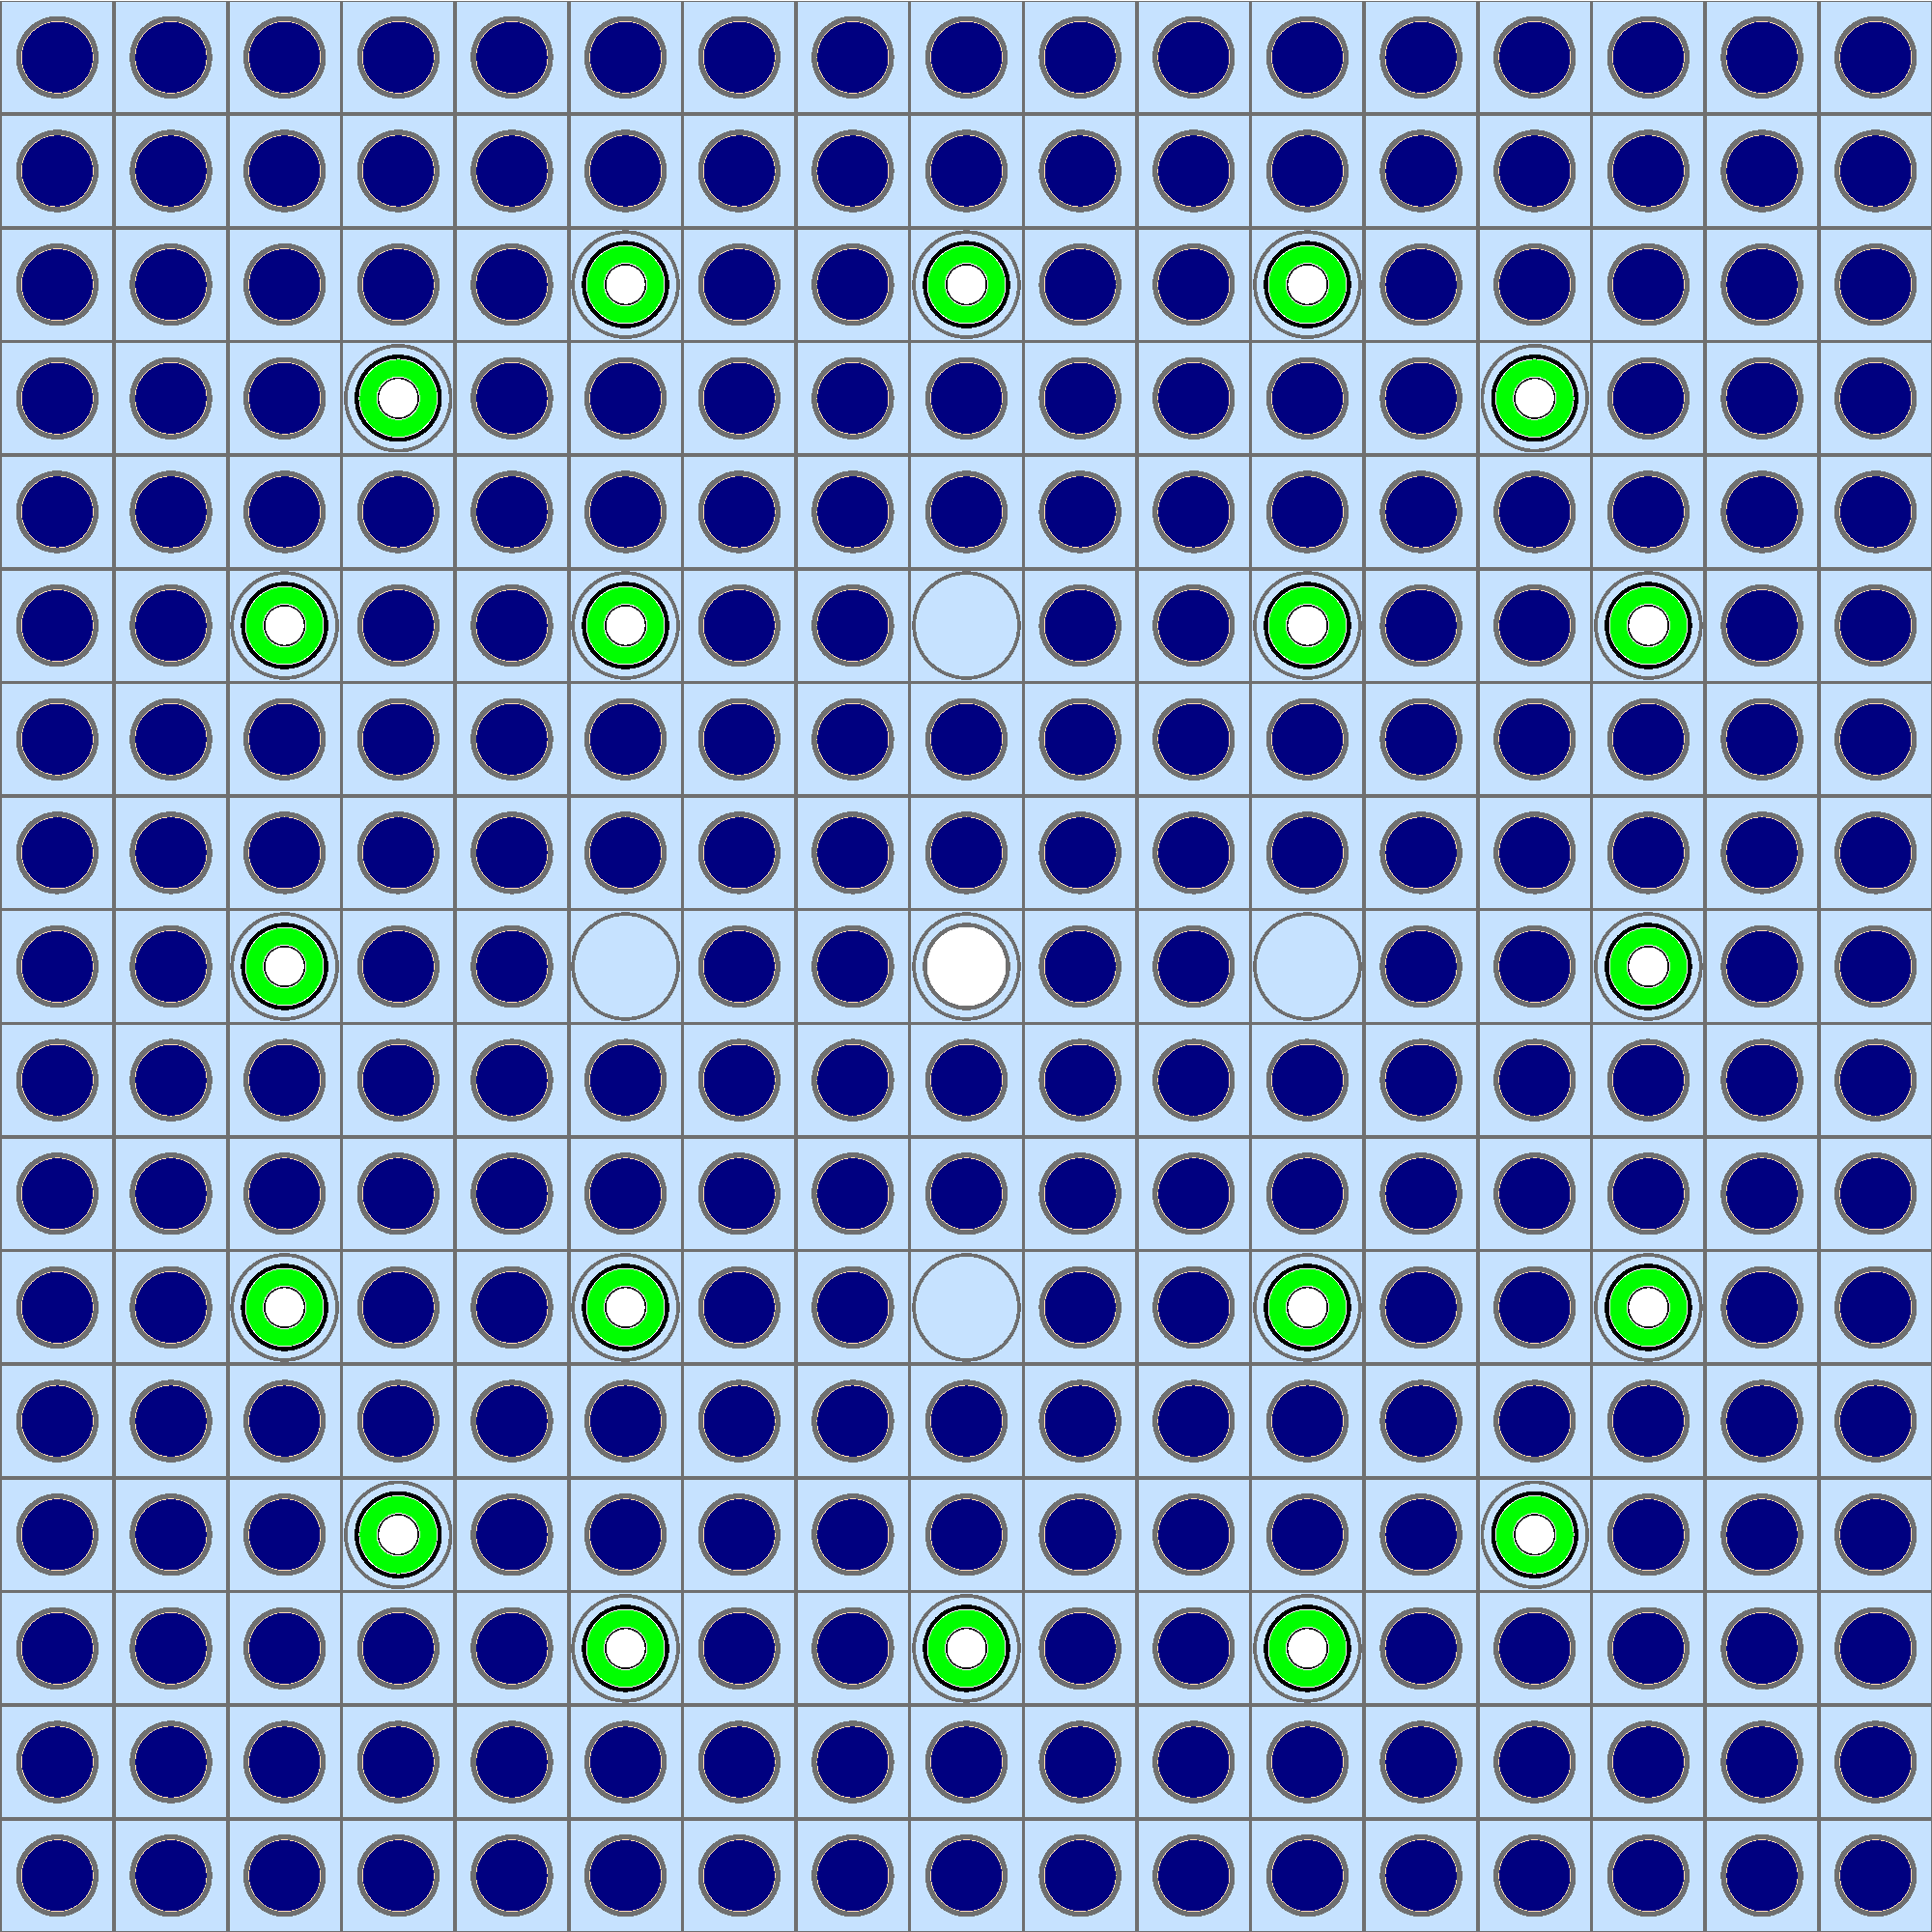
\includegraphics[width=0.65\linewidth]{figures/benchmarks/assembly-31-20BPs}
\vspace{2mm}
\caption[BEAVRS 3.1\% enriched assembly with 20 \ac{BP}s]{A 1.6\% enriched UO$_2$ fuel assembly with 20 \acp{BP}.}
\label{fig:chap7-assm-31-20BPs}
\end{figure}

The sequence of fuel assembly benchmarks are designed to investigate the impact of fuel enrichment, \acp{CRGT}, and \acp{BP} on spatially self-shielded \ac{MGXS}. The first fuel assembly benchmark depicted in Fig.~\ref{fig:chap7-assm-16} consists of 264 fuel pins with 1.6\% enriched UO$_2$ fuel, 24 \acp{CRGT}, and a single central instrument tube. The second benchmark shown in Fig.~\ref{fig:chap7-assm-31} is of the same geometric configuration, but is composed of 3.1\% enriched UO$_2$ fuel. The third benchmark illustrated in Fig.~\ref{fig:chap7-assm-31-20BPs} includes 3.1\% enriched UO$_2$ fuel with a mixture of 20 \acp{BP}, 4 \acp{CRGT} and a single central instrument tube. Although the \ac{BEAVRS} model is composed of assemblies with many different \ac{BP} configurations, only a single assembly with \acp{BP} was studied for practical reasons.

%%%%%%%%%%%%%%%%%%%%%%%%%%%%%%%%%%%%%%
\subsection{2$\times$2 Assembly Colorsets}
\label{subsec:chap7-2x2-colorsets}

Two benchmarks were constructed from 2$\times$2 colorsets of fuel assemblies from the \ac{BEAVRS} model presented in Sec.~\ref{subsec:chap7-fuel-assms}. The pitch between fuel assemblies in the colorsets is 21.41728 cm (the height/width of each assembly). The stainless steel grid sleeve and water separating each fuel assembly in the full core \ac{BEAVRS} model are not included in the 2$\times$2 colorsets. The intra-pin egg-crate grid spacer is included in each benchmark model. The first colorset is modeled with periodic \acp{BC} on all sides to simulate an infinitely repeating array of fuel assemblies. The second colorset is surrounded of a water reflector on the bottom and right that was of the same width as a fuel assembly. The reflected colorset does not include the stainless steel baffle surrounding the fuel assemblies adjacent to the water reflector in the full core \ac{BEAVRS} model. The reflected colorset includes reflective \acp{BC} on the top and left (adjacent to the fuel assemblies) with vacuum \acp{BC} on the bottom and right (adjacent to the reflector).

\begin{figure}[h!]
  \centering
  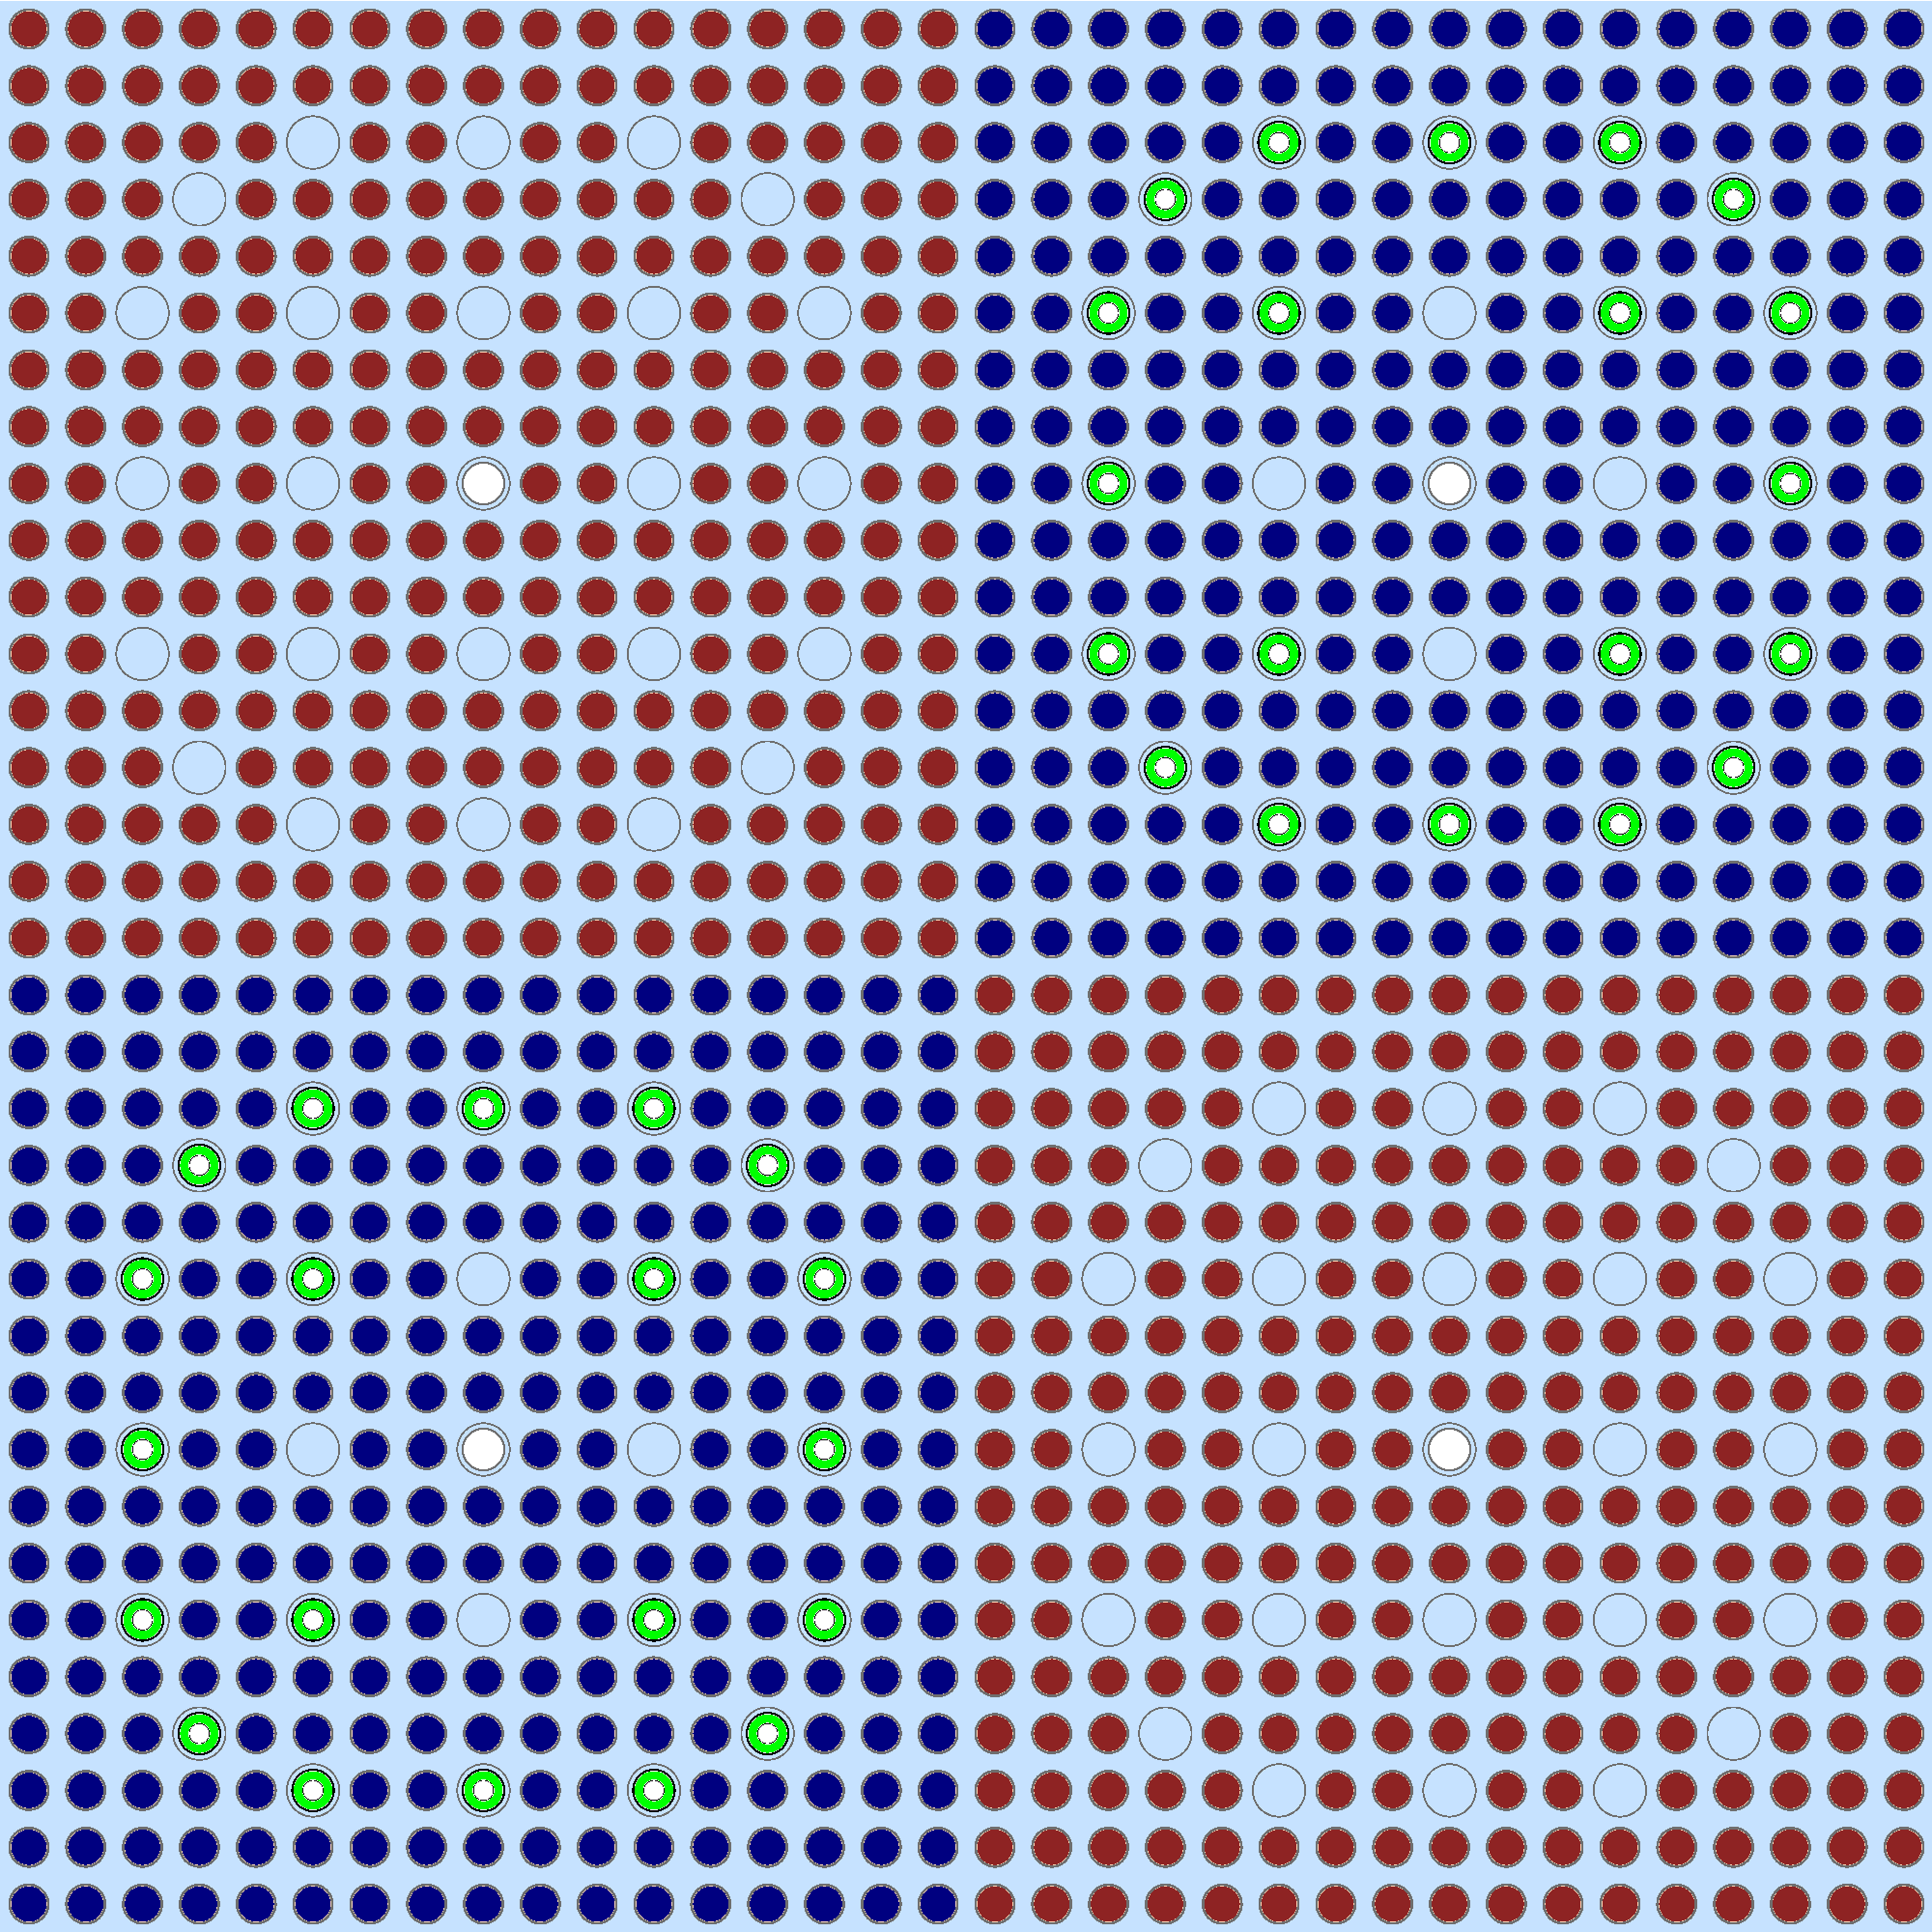
\includegraphics[width=0.63\linewidth]{figures/benchmarks/2x2}
\vspace{2mm}
\caption[A 2$\times$2 colorset of BEAVRS assemblies]{A 2$\times$2 colorset of BEAVRS assemblies with periodic \acp{BC}.}
\label{fig:chap7-2x2}
\end{figure}

\begin{figure}[h!]
  \centering
  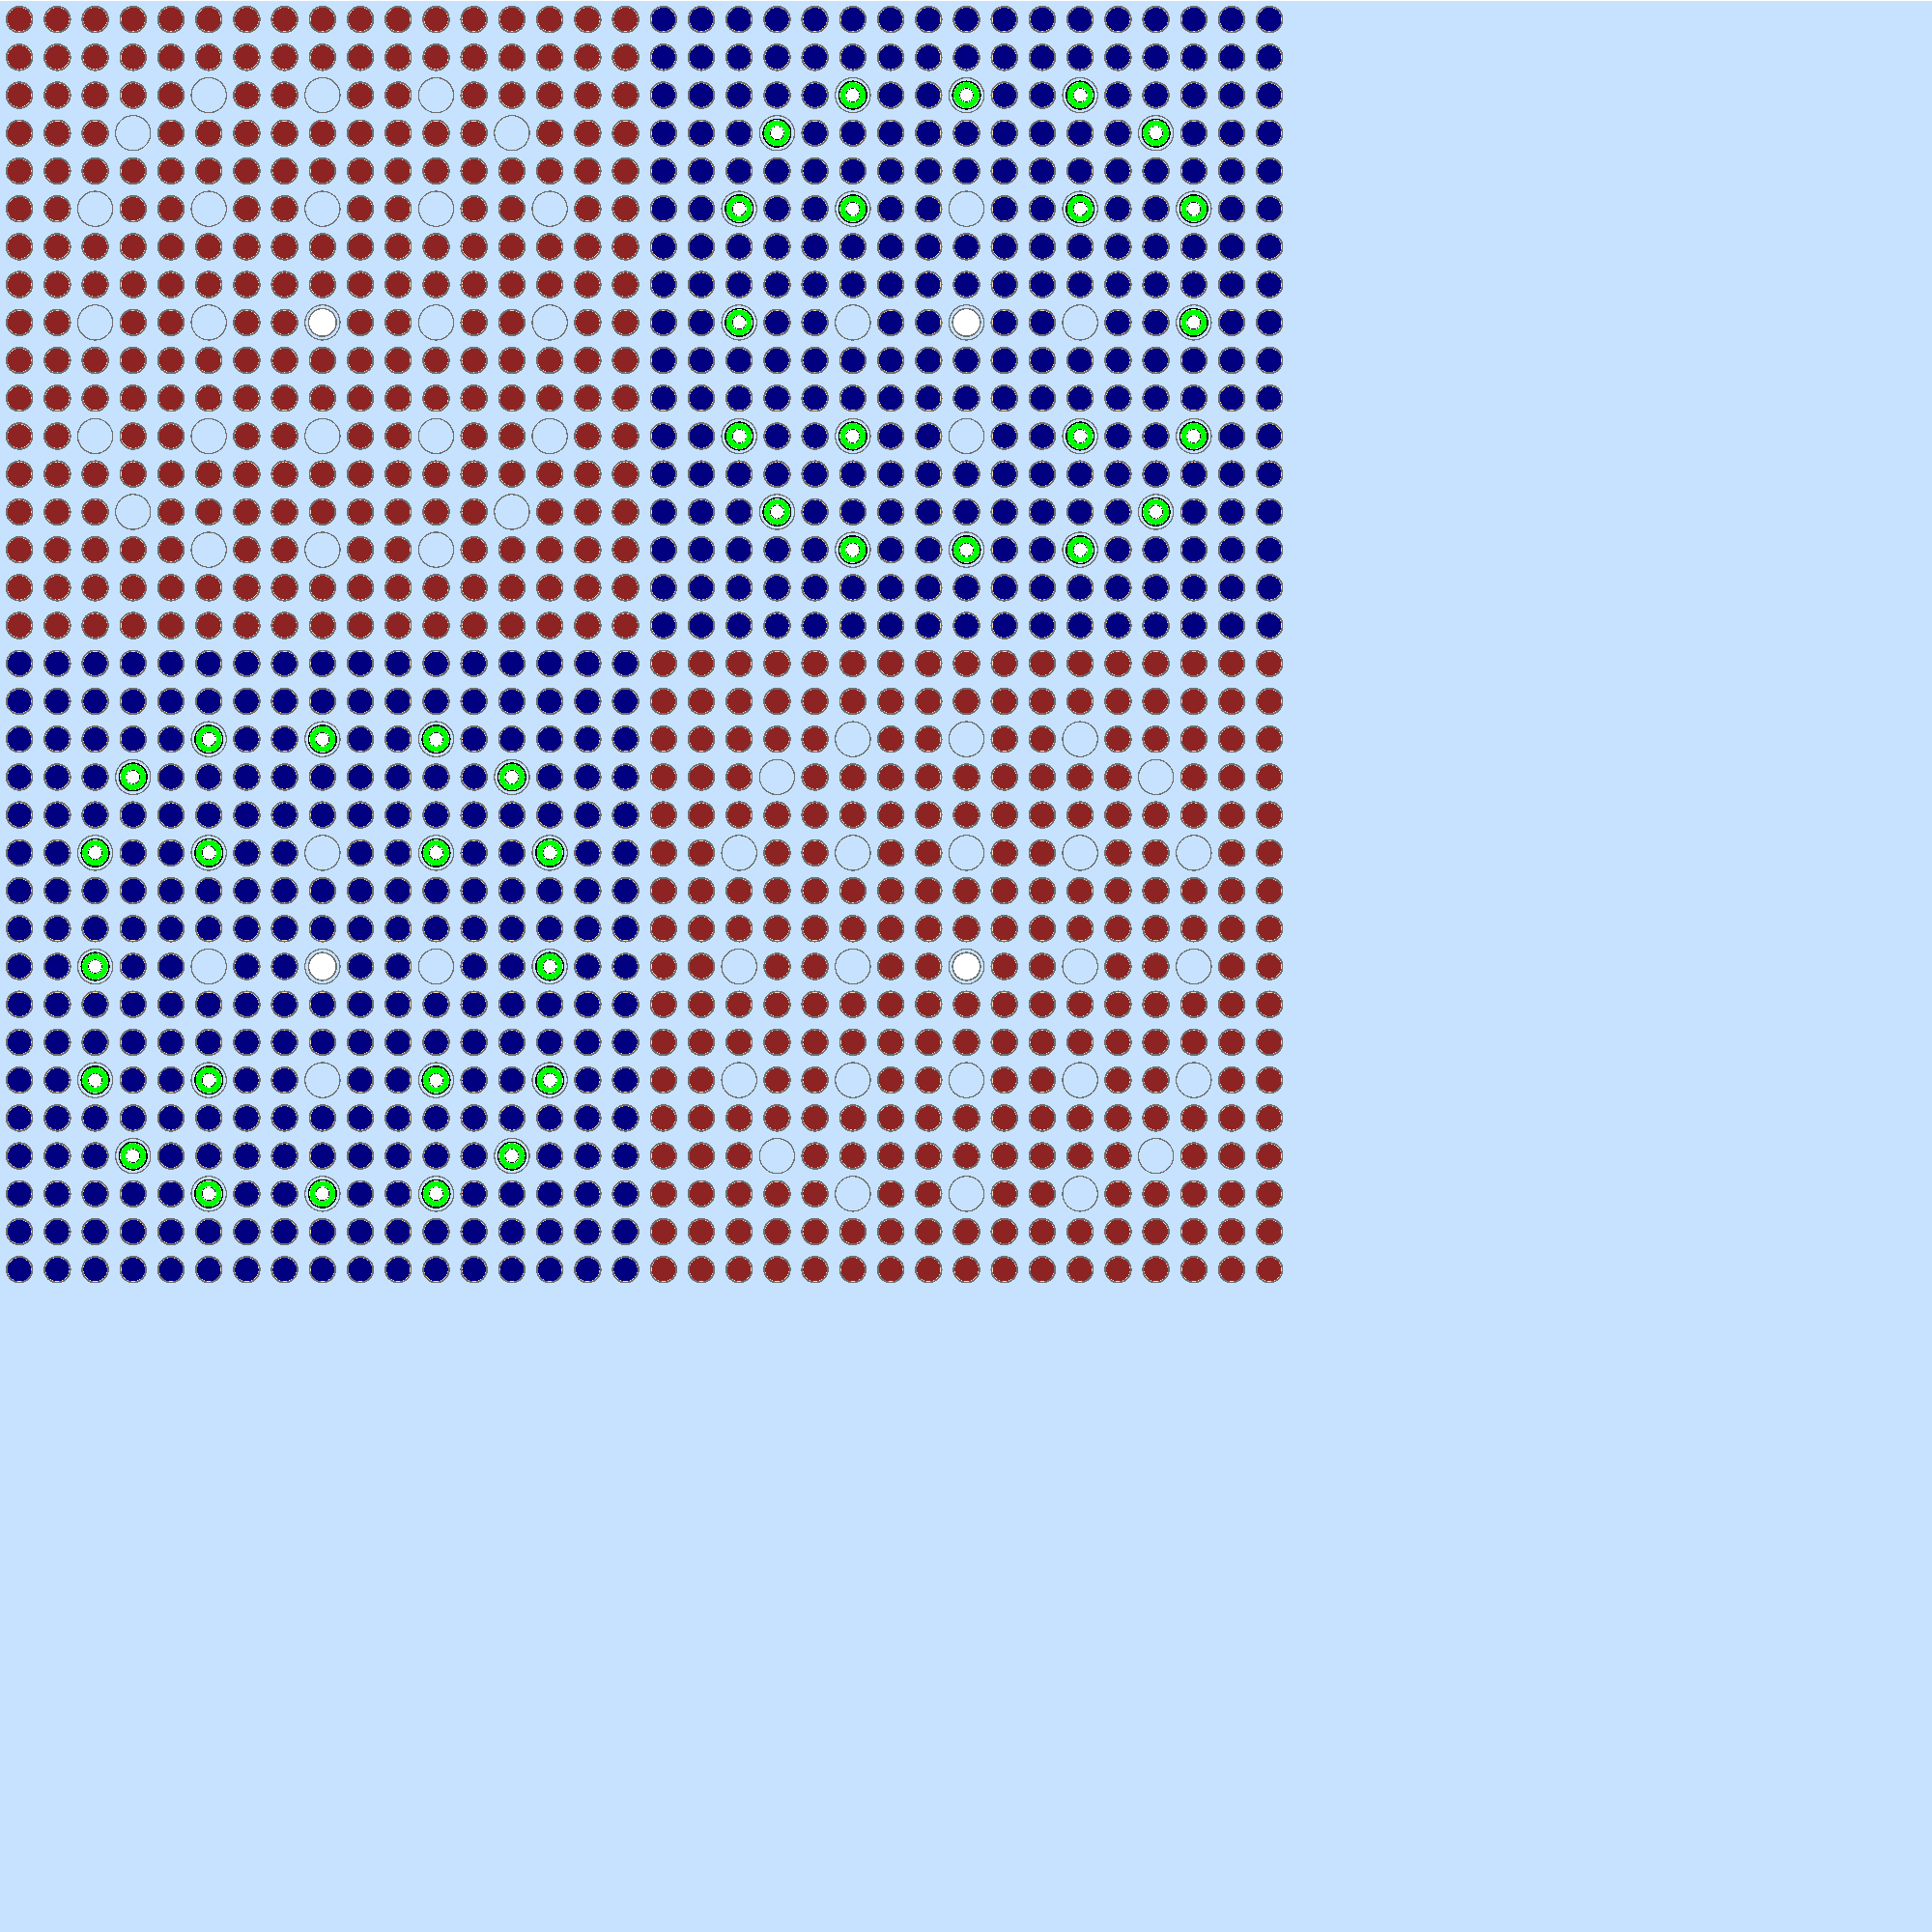
\includegraphics[width=0.63\linewidth]{figures/benchmarks/reflector}
\vspace{2mm}
\caption[A reflected 2$\times$2 colorset of BEAVRS assemblies]{A 2$\times$2 colorset of BEAVRS assemblies surrounded by a water reflector. Reflective \acp{BC} were applied on the left/top, with vacuum \acp{BC} on the right/bottom.}
\label{fig:chap7-reflector}
\end{figure}

The first 2$\times$2 colorset model shown in Fig.~\ref{fig:chap7-2x2} is composed of a checkerboard pattern of the fuel assemblies of 1.6\% enriched UO$_2$ without \acp{BP} (Fig.~\ref{fig:chap7-assm-16}) and 3.1\% enriched UO$_2$ with 20 \acp{BP} (Fig.~\ref{fig:chap7-assm-31-20BPs}). This benchmark model is designed to investigate the effects of inter-assembly spatial heterogeneities on the spatially self-shielded \ac{MGXS} of fuel pins of different enrichments (\textit{i.e.}, from different fuel assemblies) placed adjacent to one another. The second benchmark illustrated in Fig.~\ref{fig:chap7-reflector} is the same 2$\times$2 coloserset of fuel assemblies, but is surrounded by a water reflector. This benchmark is designed to quantify the impact of the moderation provided by the reflector, as well as the leakage of neutrons through the reflector, on spatially self-shielded \ac{MGXS}.

% -add baffle to benchmark

%%%%%%%%%%%%%%%%%%%%%%%%%%%%%
\subsection{BEAVRS Full Core}
\label{subsec:chap7-full-core}

The sixth and final benchmark is a 2D planar slice of the full core \ac{BEAVRS} model at the axial mid-plane as shown in Fig.~\ref{fig:chap7-full-core}. The 193 fuel assemblies in the full core model are configured according to the cycle 1 loading pattern detailed in the \ac{BEAVRS} specifications~\cite{horelik2013beavrs}. The full core model includes assemblies with 1.6\%, 2.4\% and 3.1\% enriched UO$_2$ fuel depicted as red, blue and yellow in Fig.~\ref{fig:chap7-full-core}, respectively. All of the radial heterogeneities in the \ac{BEAVRS} specifications are included in this model, including the inter-assembly stainless steel grid sleeves and water gaps, stainless steel baffle surrounding the fuel assemblies, core barrel, neutron shield panels and pressure vessel. The space outside of the pressure vessel is filled with air with vacuum \acp{BC} were applied to planar surfaces on the top, bottom, left and right. The 2D full core \ac{BEAVRS} model builds upon the preceding five simpler benchmarks to explore the impact of radial heterogeneities from a realistic core configuration on spatially self-shielded \ac{MGXS}.

\begin{figure}[h!]
  \centering
  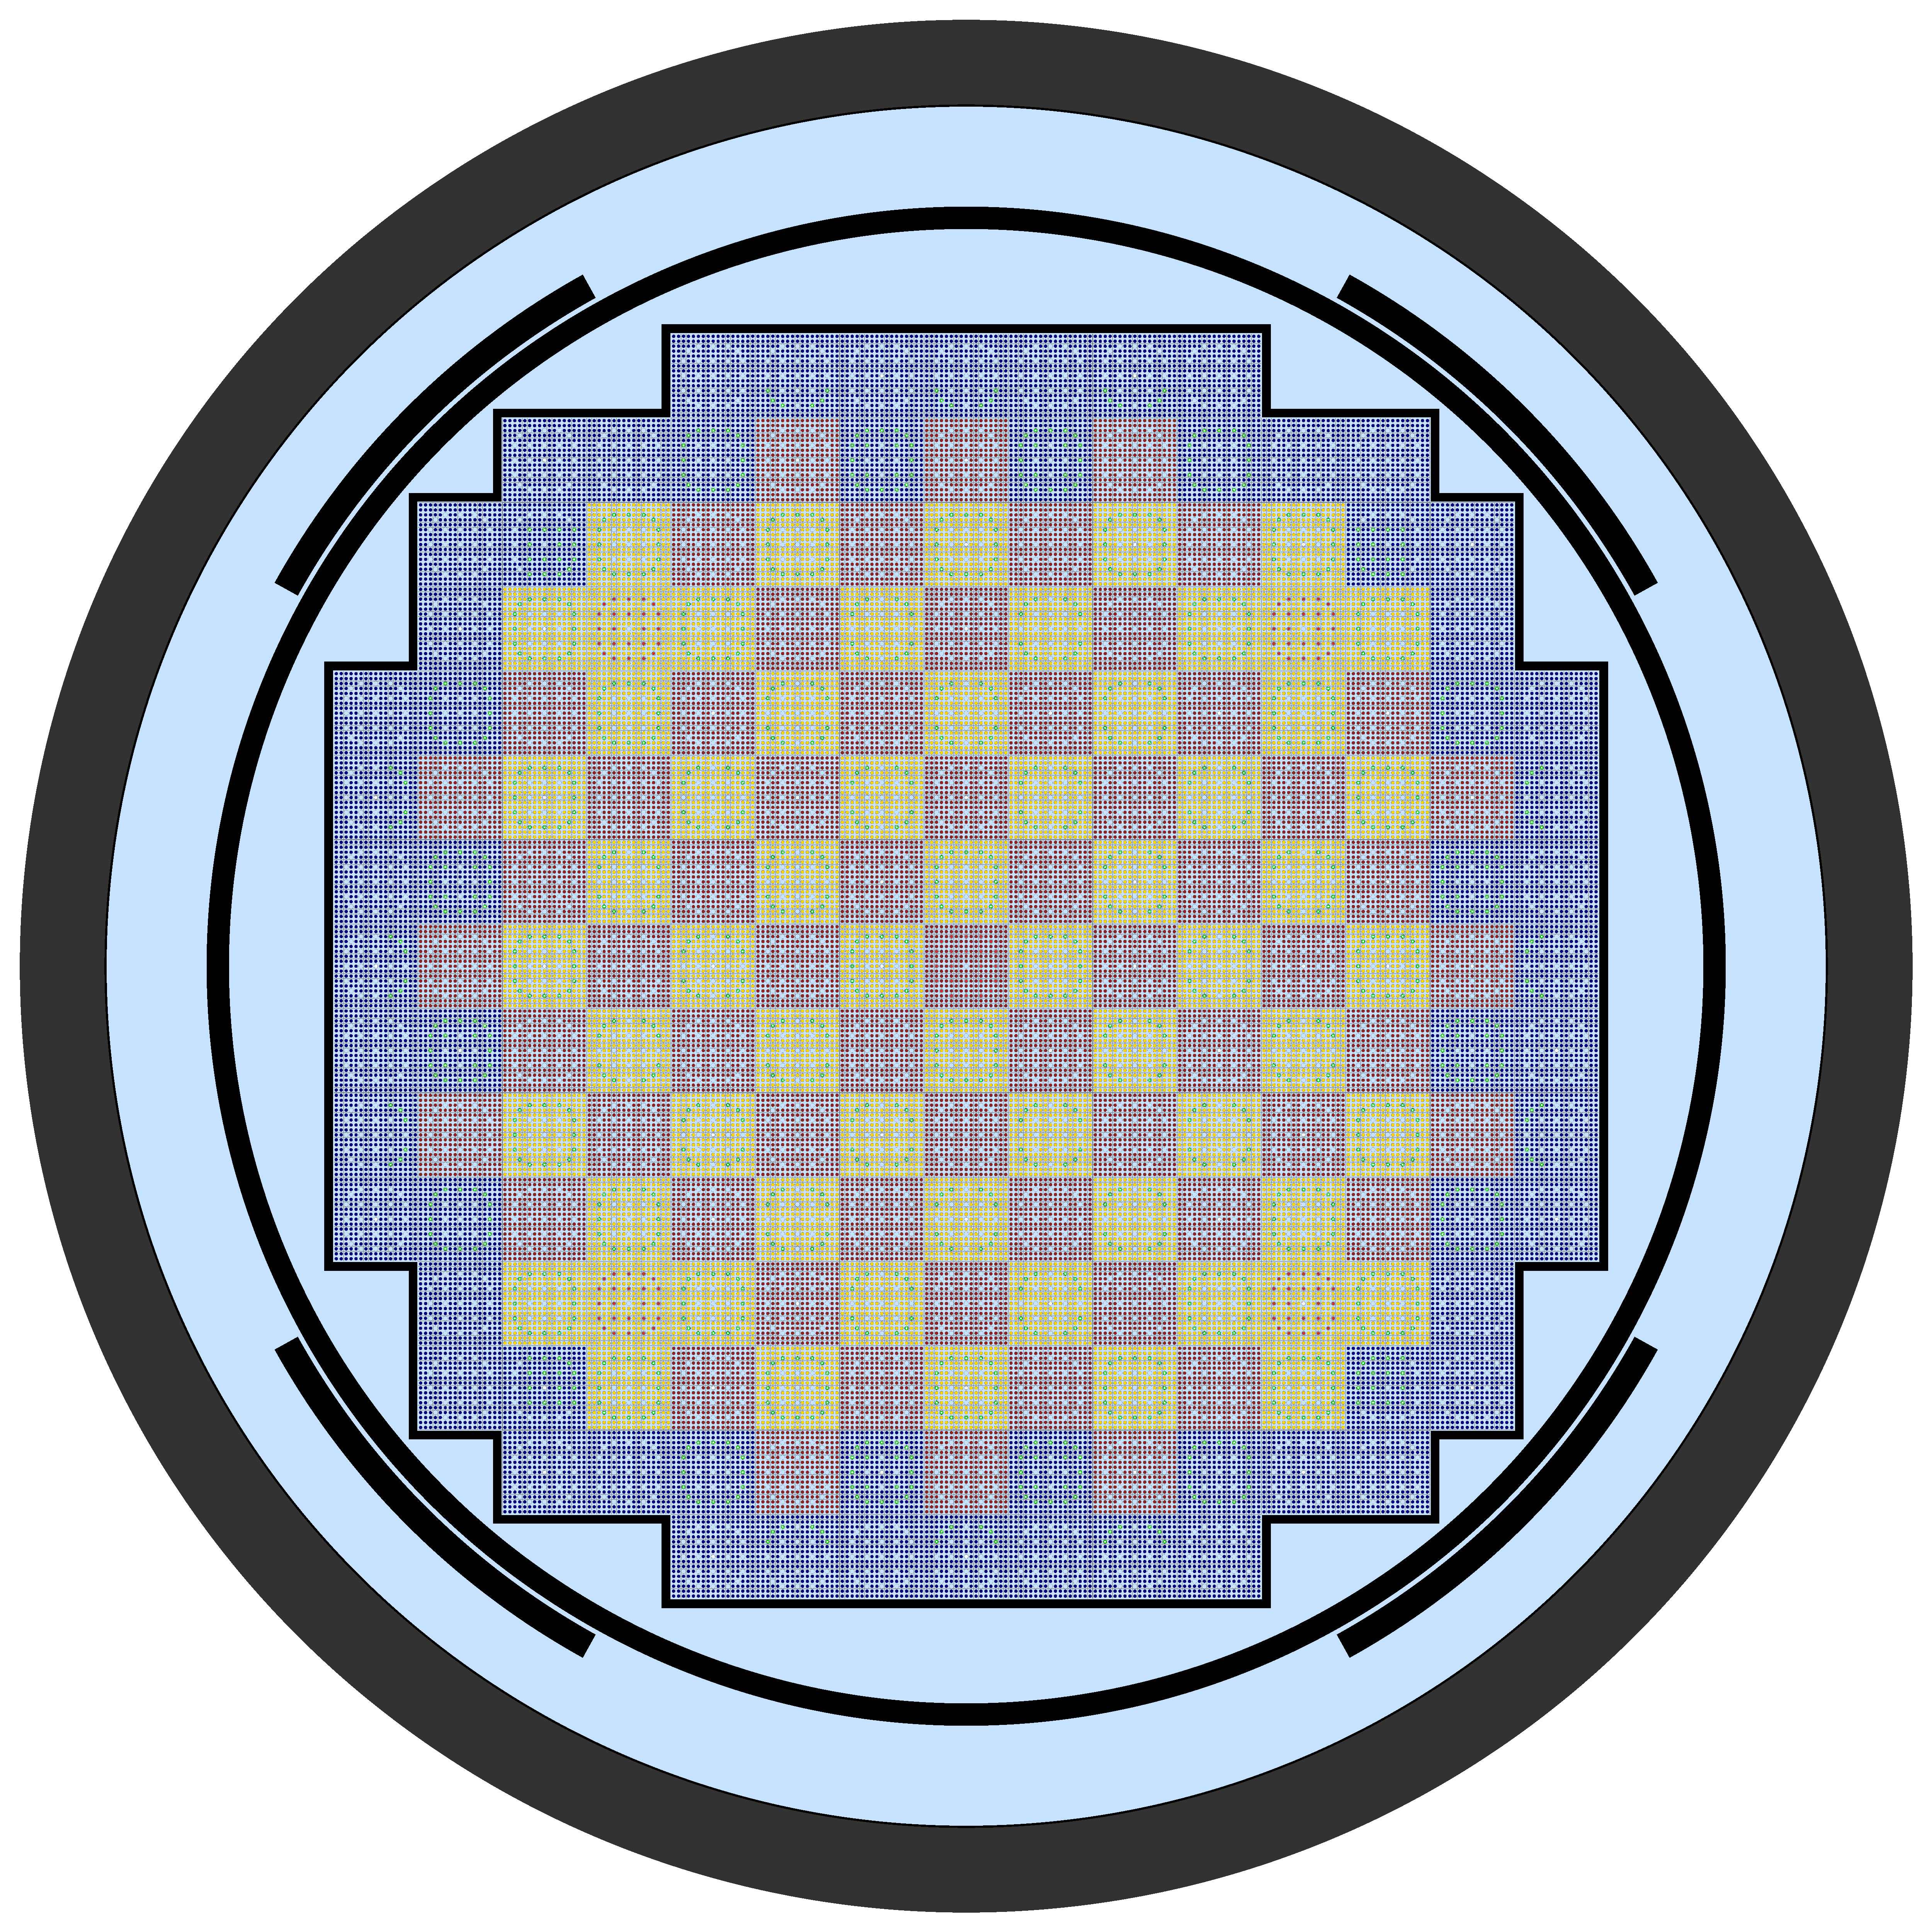
\includegraphics[width=0.9\linewidth]{figures/benchmarks/full-core}
\vspace{2mm}
\caption[The 2D full core \ac{BEAVRS} model]{The 2D full core \ac{BEAVRS} model.}
\label{fig:chap7-full-core}
\end{figure}


%%%%%%%%%%%%%%%%%%%%%%%%%%%%%%%%%%%%%%%%%%%%%%%%%%%%%%%%%%%%%%%%%%%%%%%%%%%%%%%
\section{Reference Results}
\label{sec:chap7-ref-results}

-mention iso-in-lab
-NNDC cross sections
  -not looking for truly accurate results
  -generating reference results for comparison with multi-group \ac{MOC}
-metrics of interest:
  -eigenvalue
  -energy-integrated pin-wise fission rates using an OpenMC rectilinear mesh tally
  -energy-integrated pin-wise U-238 capture rates using an OpenMC rectilinear mesh tally
 
runtime parameters:
-1000 total batches
  -200 inactive batches
  -800 active batches
-5 nodes of 24 Intel Xeon cores each
-2 MPI processes per node
-12 OpenMP threads per MPI process

%%%%%%%%%%%%%%%%%%%%%%%%%%%%%%%
\subsection{Source Convergence}
\label{subsec:chap7-src-converge}

first paragraph: shannon entropy
-reference for shannon entropy to indicate source stationarity (Herman's thesis??)
-pin-wise entropy mesh, used OpenMC's internally calculated shannon entropy
-need to determine \# batches to reach reasonable source stationarity
-used to fix the number of inactive batches before tallying 

second paragraph:
-Fig.~\ref{fig:chap7-entropy} - convergence of entropy for each of the benchmarks
-normalized entropy to the final value on the last batch
-stationary entropy is different for each geometry
-normalization makes it easy to compare entropies for each benchmark
-trivial convergence for individual fuel assemblies
-takes $\sim$10 batches for the 2$\times$2 with reflector to converge
-takes $\sim$200 batches for the full core \ac{BEAVRS} to converge
-will use 100 inactive batches for all fuel assembly and 2$\times$ colorsets in subsequent simulations
-will use 200 inactive batches for all full core \ac{BEAVRS} simulations in subsequent simulations

\begin{figure}[h!]
  \centering
  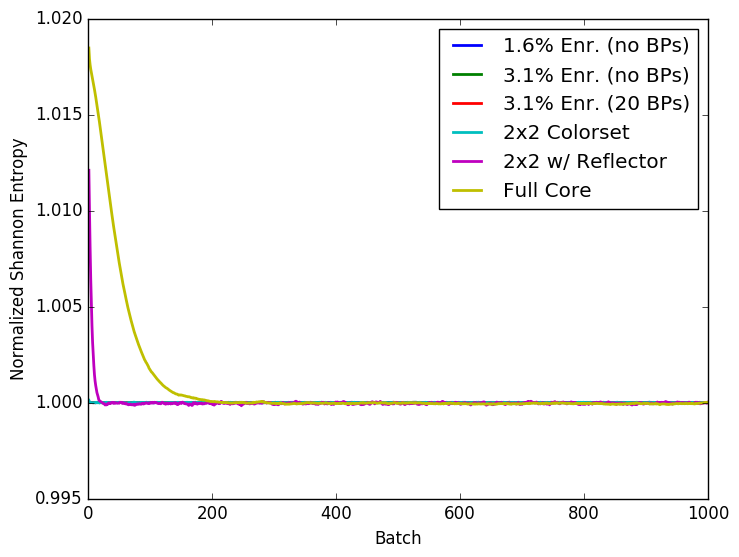
\includegraphics[width=0.9\linewidth]{figures/benchmarks/entropy/entropy-all}
\caption[Shannon entropy source convergence for BEAVRS geometries]{Shannon entropy source convergence for BEAVRS geometries.}
\label{fig:chap7-entropy}
\end{figure}


%%%%%%%%%%%%%%%%%%%%%%%%
\subsection{Eigenvalues}
\label{subsec:chap7-eigenvalues}

first paragraph: eigenvalues
-Tab.~\ref{table:chap7-ref-eigenvalues} - converged eigenvalues for each benchmark
-total runtime in CPU-hours for each case
  -used same \# batches, \# particle histories / batch
  -variation due to varying complexity of tracking particles in different geometries
-trends
  -greater enrichment (1.6\% to 3.1\%) increases fission-to-absorption ratio and increases eigenvalue
  -\ac{BP}s increases absorption and reduces eigenvalue
  -reflector reduces eigenvalue due to absorption and leakage
-final converged eigenvalues serve as the reference for each benchmark throughout the remainder of thesis

\begin{table}[h!]
  \centering
  \caption[Reference $k^{OpenMC}_{eff}$ for heterogeneous benchmarks]{Reference $k^{OpenMC}_{eff}$ for heterogeneous benchmarks.}
  \small
  \label{table:chap7-ref-eigenvalues}
  \vspace{6pt}
  \begin{tabular}{l C{4cm} c}
  \toprule
  \rowcolor{lightgray}
  \textbf{Benchmark} & $\bm{k^{OpenMC}_{eff}}$ & \textbf{Runtime [CPU-hours]} \\
  \midrule
  1.6\% Enriched Assembly (no \ac{BP}s) & 1.00987 $\pm$ 0.00003 & 331 \\
  3.1\% Enriched Assembly (no \ac{BP}s) & 1.22344 $\pm$ 0.00003 & 326 \\
  3.1\% Enriched Assembly (20 \ac{BP}s) & 1.04530 $\pm$ 0.00003 & 331 \\
  2$\times$2 Colorset & 1.03196 $\pm$ 0.00003 & 345 \\
  2$\times$2 Colorset w/ Reflector & 0.95462 $\pm$ 0.00003 & 337 \\
  \ac{BEAVRS} Full Core & 1.02497 $\pm$ 0.00003 & 387 \\
  \bottomrule
\end{tabular}
\end{table}

%%%%%%%%%%%%%%%%%%%%%%%%%%%%%%%%%%%%
\subsection{Fission Rate Spatial Distributions}
\label{subsec:chap7-pin-powers}

first paragraph: fission rates
-how they were computed 
  -rectilinear tally mesh in OpenMC
  -energy-integrated
  -volume-integrated across each pin
  -fission from all nuclides
-relative error or uncertainty computed how???

second paragraph: spatial distributions
-Fig.~\Crefrange{fig:chap7-fiss-rates-1.6-assm}{fig:chap7-fiss-rates-full-core} - all benchmark geometries
-trends:
  -adjacency to \ac{CRGT}s provides added moderation and increases fission rates
  -adjacency to \ac{BP}s reduces neutron population and reduces fission rates
  -pins in 3.1\% assm in 2$\times$2 have $\sim$35\% higher fission rates than those in 1.6\% assm
    -more peaking / variation due to \ac{BP}s
  -adjacency to reflector reduces fission rates since leakage reduces neutrons
  -full core has complex distribution of fission rates

third paragraph: convergence rate
-Fig.~\ref{fig:chap7-fiss-rates-conv} has convergence of fission rate uncertainties
-well below 1\% uncertainty of fission rates in each pin for 2D \ac{BEAVRS} benchmark
-smoother convergence for mean than for max

\begin{figure}[h!]
\centering
\begin{subfigure}{0.5\textwidth}
  \centering
  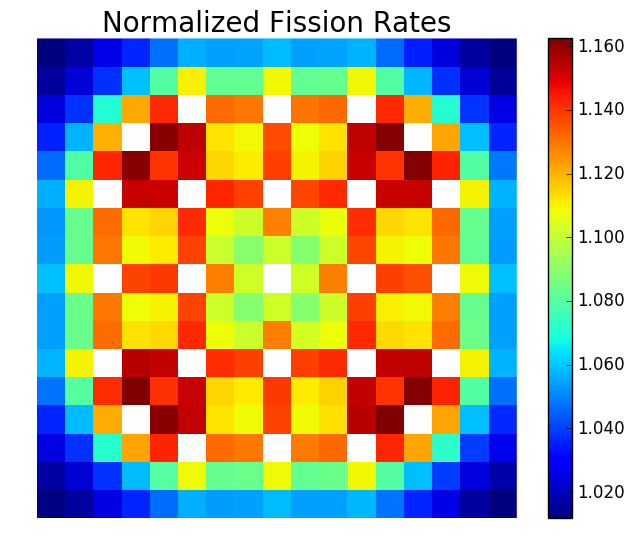
\includegraphics[width=\linewidth]{figures/benchmarks/fission-rates/fiss-mean-fuel-16}
  \caption{}
  \label{fig:chap7-fiss-rate-mean-1.6-assm}
\end{subfigure}%
\begin{subfigure}{0.5\textwidth}
  \centering
  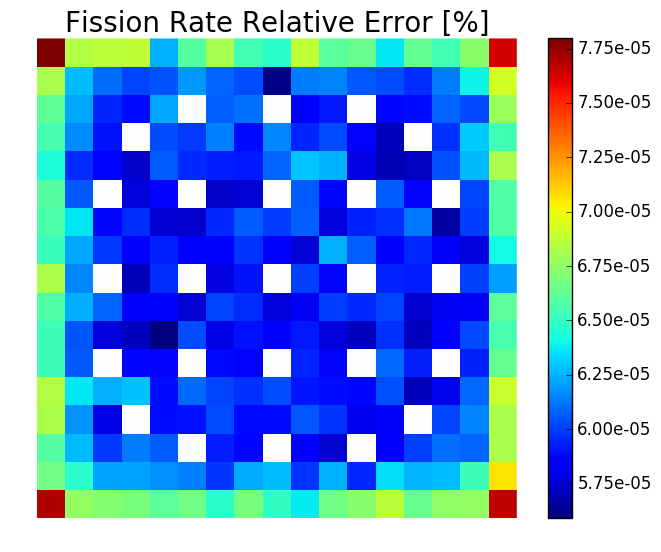
\includegraphics[width=\linewidth]{figures/benchmarks/fission-rates/fiss-rel-err-fuel-16}
  \caption{}
  \label{fig:chap7-fiss-rate-rel-err-1.6-assm}
\end{subfigure}%
\caption[Fission rates for a 1.6\% enriched assembly]{Fission rates for a 1.6\% enriched assembly.}
\label{fig:chap7-fiss-rates-1.6-assm}
\end{figure}

\begin{figure}[h!]
\centering
\begin{subfigure}{0.5\textwidth}
  \centering
  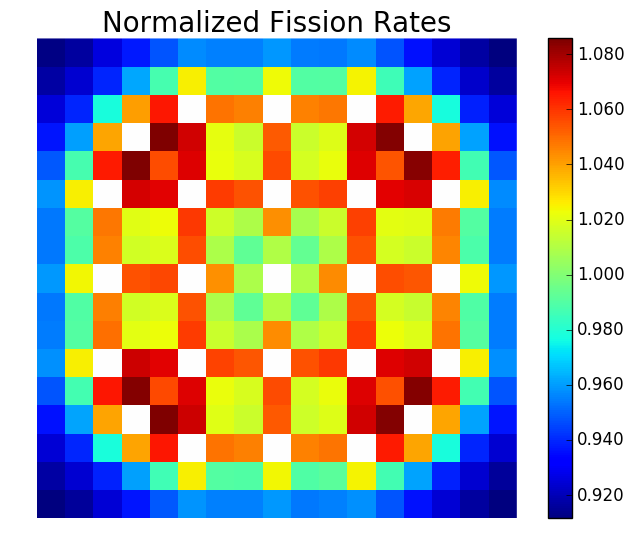
\includegraphics[width=\linewidth]{figures/benchmarks/fission-rates/fiss-mean-fuel-31}
  \caption{}
  \label{fig:chap7-fiss-rate-mean-3.1-assm}
\end{subfigure}%
\begin{subfigure}{0.5\textwidth}
  \centering
  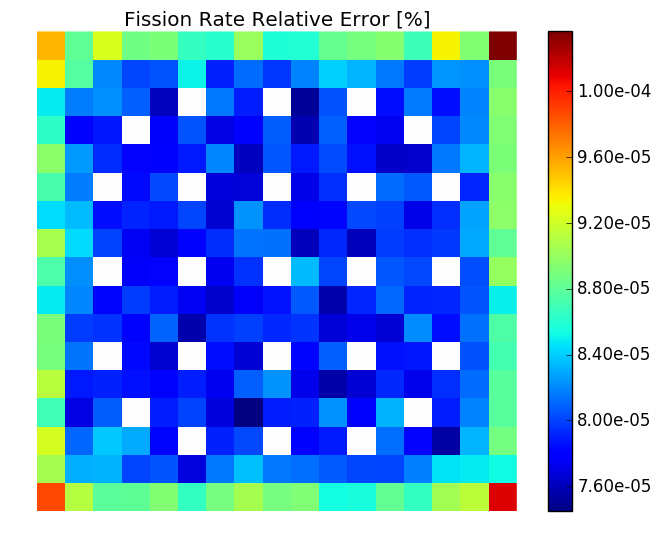
\includegraphics[width=\linewidth]{figures/benchmarks/fission-rates/fiss-rel-err-fuel-31}
  \caption{}
  \label{fig:chap7-fiss-rate-rel-err-3.1-assm}
\end{subfigure}%
\caption[Fission rates for a 3.1\% enriched assembly]{Fission rates for a 3.1\% enriched assembly.}
\label{fig:chap7-fiss-rates-3.1-assm}
\end{figure}

\begin{figure}[h!]
\centering
\begin{subfigure}{0.5\textwidth}
  \centering
  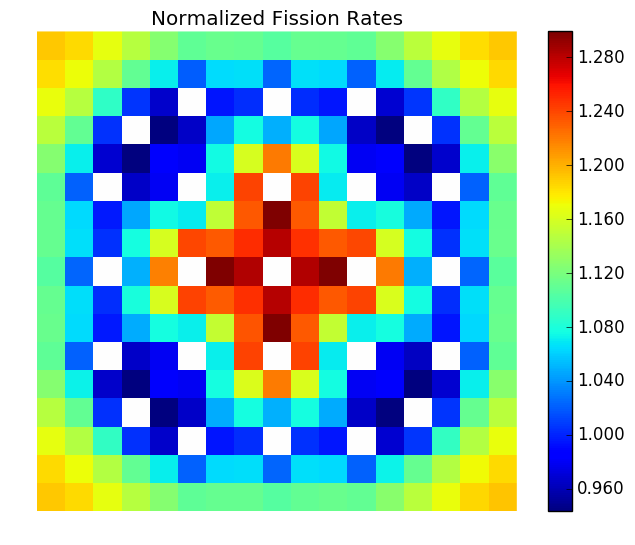
\includegraphics[width=\linewidth]{figures/benchmarks/fission-rates/fiss-mean-fuel-31-20BAs}
  \caption{}
  \label{fig:chap7-fiss-rate-mean-3.1-20BAs-assm}
\end{subfigure}%
\begin{subfigure}{0.5\textwidth}
  \centering
  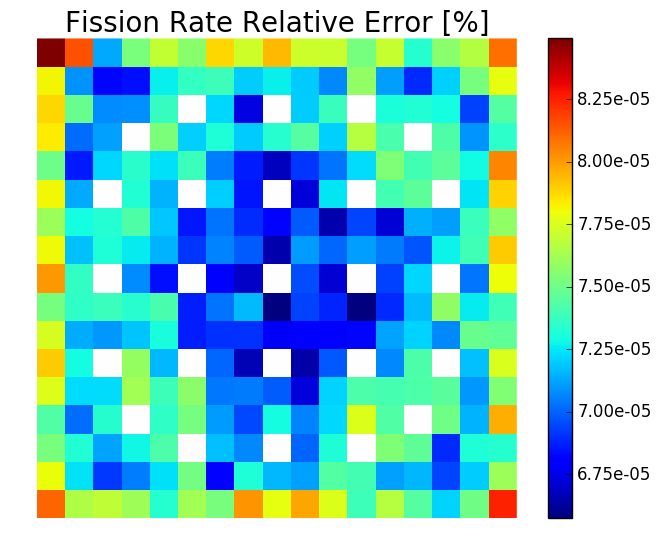
\includegraphics[width=\linewidth]{figures/benchmarks/fission-rates/fiss-rel-err-fuel-31-20BAs}
  \caption{}
  \label{fig:chap7-fiss-rate-rel-err-3.1-20BAs-assm}
\end{subfigure}%
\caption[Fission rates for a 3.1\% enriched assembly with 20 BPs]{Fission rates for a 3.1\% enriched assembly with 20 \ac{BP}s.}
\label{fig:chap7-fiss-rates-3.1-assm-20BAs}
\end{figure}

\begin{figure}[h!]
\centering
\begin{subfigure}{0.5\textwidth}
  \centering
  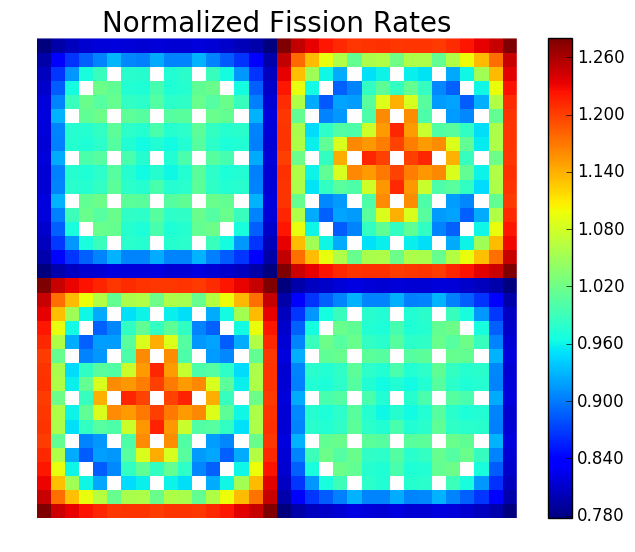
\includegraphics[width=\linewidth]{figures/benchmarks/fission-rates/fiss-mean-2x2}
  \caption{}
  \label{fig:chap7-fiss-rate-mean-2x2}
\end{subfigure}%
\begin{subfigure}{0.5\textwidth}
  \centering
  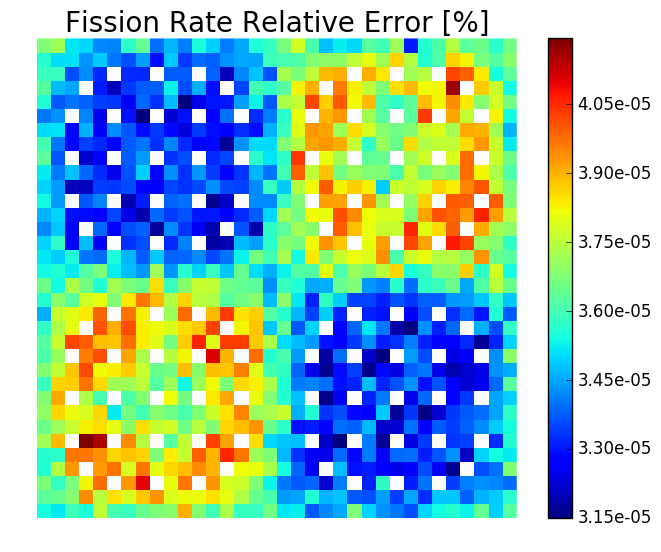
\includegraphics[width=\linewidth]{figures/benchmarks/fission-rates/fiss-rel-err-2x2}
  \caption{}
  \label{fig:chap7-fiss-rate-rel-err-2x2}
\end{subfigure}%
\caption[Fission rates for a 2$\times$2 colorset]{Fission rates for a 2$\times$2 colorset.}
\label{fig:chap7-fiss-rates-2x2}
\end{figure}

\begin{figure}[h!]
\centering
\begin{subfigure}{0.5\textwidth}
  \centering
  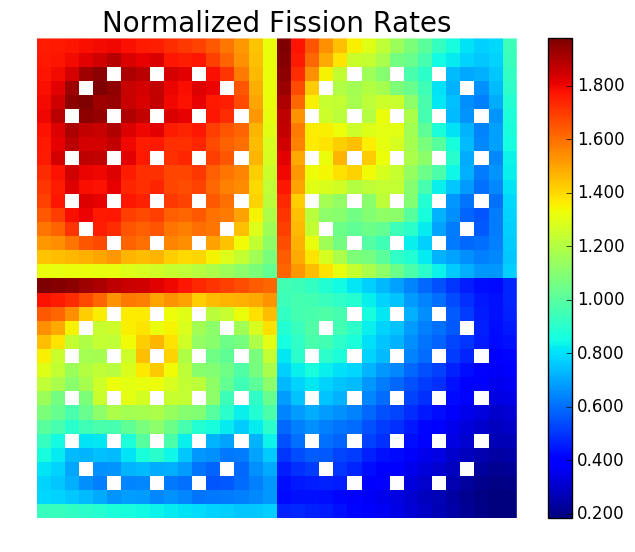
\includegraphics[width=\linewidth]{figures/benchmarks/fission-rates/fiss-mean-reflector}
  \caption{}
  \label{fig:chap7-fiss-rate-conv}
\end{subfigure}%
\begin{subfigure}{0.5\textwidth}
  \centering
  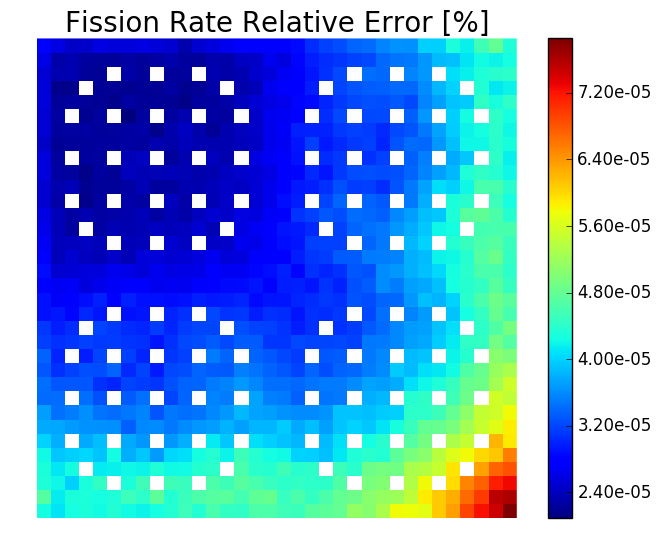
\includegraphics[width=\linewidth]{figures/benchmarks/fission-rates/fiss-rel-err-reflector}
  \caption{}
  \label{fig:chap7-fiss-rate-conv}
\end{subfigure}%
\caption[Fission rates for a 2$\times$2 colorset with a reflector]{Fission rates for a 2$\times$2 colorset with a reflector.}
\label{fig:chap7-fiss-rates-2x2}
\end{figure}

\begin{figure}[h!]
\centering
\begin{subfigure}{0.5\textwidth}
  \centering
  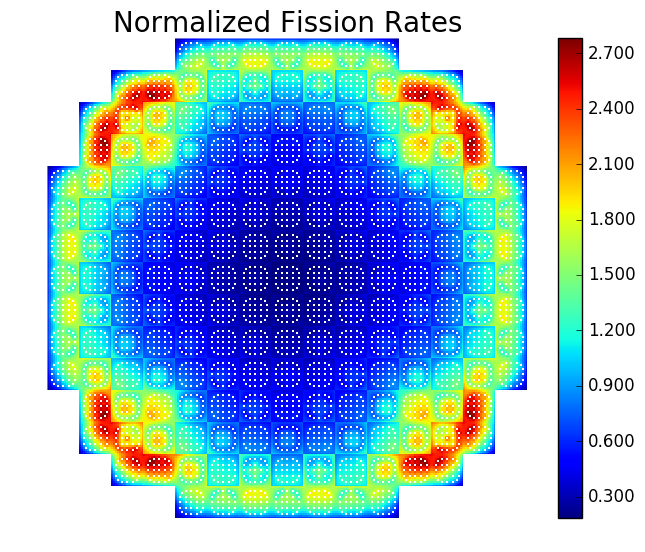
\includegraphics[width=\linewidth]{figures/benchmarks/fission-rates/fiss-mean-full-core}
  \caption{}
  \label{fig:chap7-fiss-rate-mean-full-core}
\end{subfigure}%
\begin{subfigure}{0.5\textwidth}
  \centering
  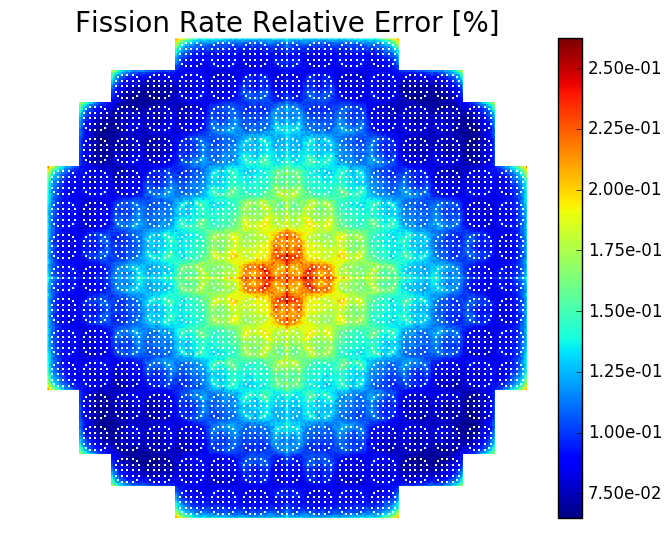
\includegraphics[width=\linewidth]{figures/benchmarks/fission-rates/fiss-rel-err-full-core}
  \caption{}
  \label{fig:chap7-fiss-rate-rel-err-full-core}
\end{subfigure}%
\caption[Fission rates for the full 2D BEAVRS core]{Fission rates for the full 2D \ac{BEAVRS} core.}
\label{fig:chap7-fiss-rates-full-core}
\end{figure}

\begin{figure}[h!]
\centering
\begin{subfigure}{\textwidth}
  \centering
  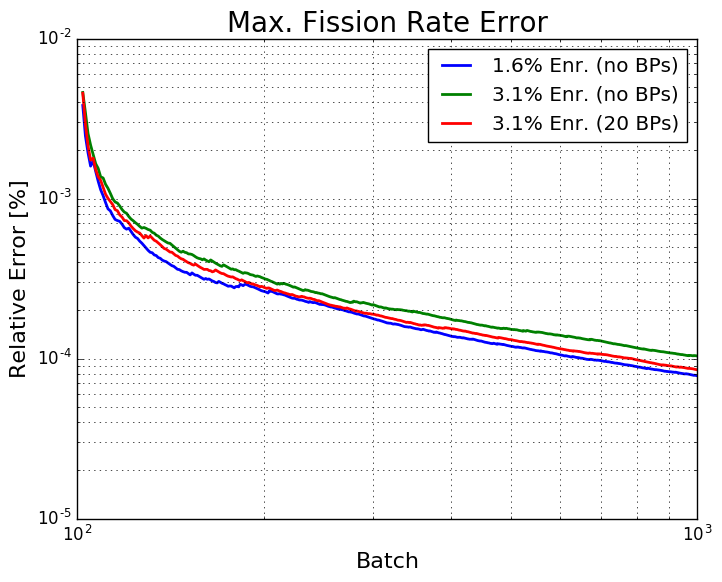
\includegraphics[width=0.8\linewidth]{figures/benchmarks/fission-rates/fiss-conv-max-assms}
  \caption{}
  \label{fig:chap7-fiss-rate-max-conv-max}
\end{subfigure}
\begin{subfigure}{\textwidth}
  \centering
  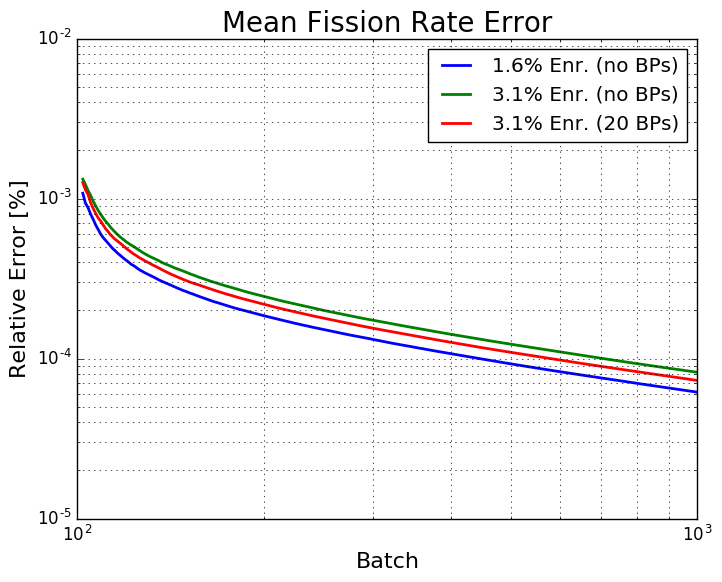
\includegraphics[width=0.8\linewidth]{figures/benchmarks/fission-rates/fiss-conv-mean-assms}
  \caption{}
  \label{fig:chap7-fiss-rate-max-conv-mean}
\end{subfigure}
\caption[Fission rate error convergence for BEAVRS geometries]{Fission rate relative error convergence for \ac{BEAVRS} geometries.}
\label{fig:chap7-fiss-rates-conv}
\end{figure}

%%%%%%%%%%%%%%%%%%%%%%%%%%%%%%%%%%%%%%%%%%%%%
\subsection{U-238 Capture Rate Spatial Distributions}
\label{subsec:chap7-capture-rates}

first paragraph: U-238 capture rates
-how they were computed 
  -rectilinear tally mesh in OpenMC
  -energy-integrated
  -volume-integrated across each pin
  -only for U-238
-relative error or uncertainty computed how???

second paragraph: spatial distributions
-Fig.~\Crefrange{fig:chap7-capt-rates-1.6-assm}{fig:chap7-capt-rates-full-core} - all benchmark geometries
-trends - similar to fission rates since U-238 capture dominated by low-lying resonances
  -adjacency to \ac{CRGT}s provides added moderation and increases capture rates
  -adjacency to \ac{BP}s reduces neutron population and reduces capture rates
  -pins in 3.1\% assm in 2$\times$2 have $\sim$35\% higher capture rates than those in 1.6\% assm
    -more peaking / variation due to \ac{BP}s
  -adjacency to reflector reduces capture rates since leakage reduces neutrons
  -full core has complex distribution of capture rates

third paragraph: convergence rate
-Fig.~\ref{fig:chap7-capt-rates-conv} has convergence of capture rate uncertainties
-well below 1\% uncertainty of capture rates in each pin for 2D \ac{BEAVRS} benchmark
-smoother convergence for mean than for max

\begin{figure}[h!]
\centering
\begin{subfigure}{0.5\textwidth}
  \centering
  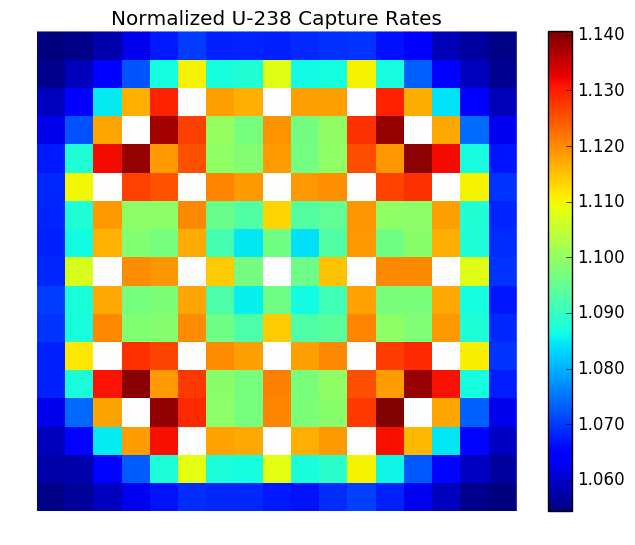
\includegraphics[width=\linewidth]{figures/benchmarks/capture-rates/capt-mean-fuel-16}
  \caption{}
  \label{fig:chap7-capt-rate-mean-1.6-assm}
\end{subfigure}%
\begin{subfigure}{0.5\textwidth}
  \centering
  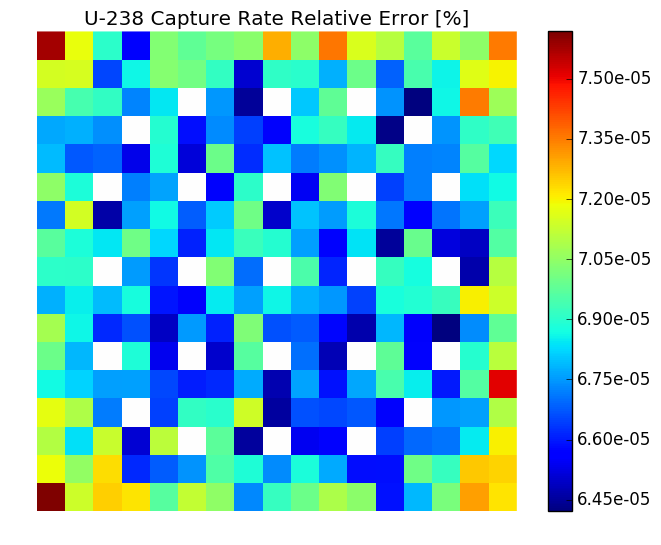
\includegraphics[width=\linewidth]{figures/benchmarks/capture-rates/capt-rel-err-fuel-16}
  \caption{}
  \label{fig:chap7-capt-rate-rel-err-1.6-assm}
\end{subfigure}%
\caption[U-238 capture rates for a 1.6\% enriched assembly]{U-238 capture rates for a 1.6\% enriched assembly.}
\label{fig:chap7-capt-rates-1.6-assm}
\end{figure}

\begin{figure}[h!]
\centering
\begin{subfigure}{0.5\textwidth}
  \centering
  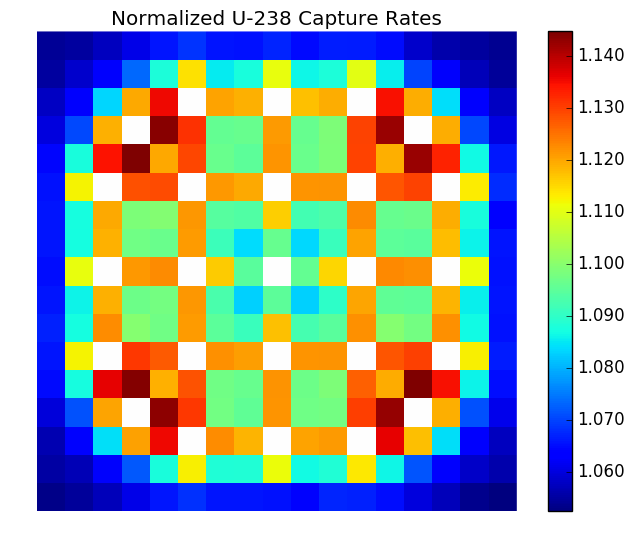
\includegraphics[width=\linewidth]{figures/benchmarks/capture-rates/capt-mean-fuel-31}
  \caption{}
  \label{fig:chap7-capt-rate-mean-3.1-assm}
\end{subfigure}%
\begin{subfigure}{0.5\textwidth}
  \centering
  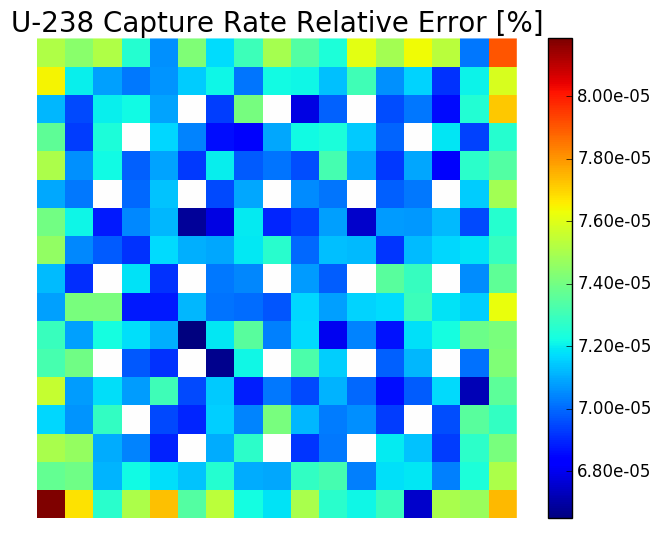
\includegraphics[width=\linewidth]{figures/benchmarks/capture-rates/capt-rel-err-fuel-31}
  \caption{}
  \label{fig:chap7-capt-rate-rel-err-3.1-assm}
\end{subfigure}%
\caption[U-238 capture rates for a 3.1\% enriched assembly]{U-238 capture rates for a 3.1\% enriched assembly.}
\label{fig:chap7-capt-rates-3.1-assm}
\end{figure}

\begin{figure}[h!]
\centering
\begin{subfigure}{0.5\textwidth}
  \centering
  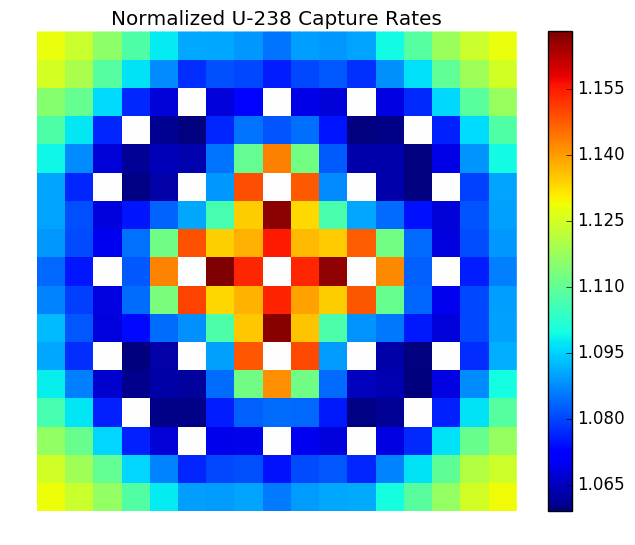
\includegraphics[width=\linewidth]{figures/benchmarks/capture-rates/capt-mean-fuel-31-20BAs}
  \caption{}
  \label{fig:chap7-capt-rate-mean-3.1-20BAs-assm}
\end{subfigure}%
\begin{subfigure}{0.5\textwidth}
  \centering
  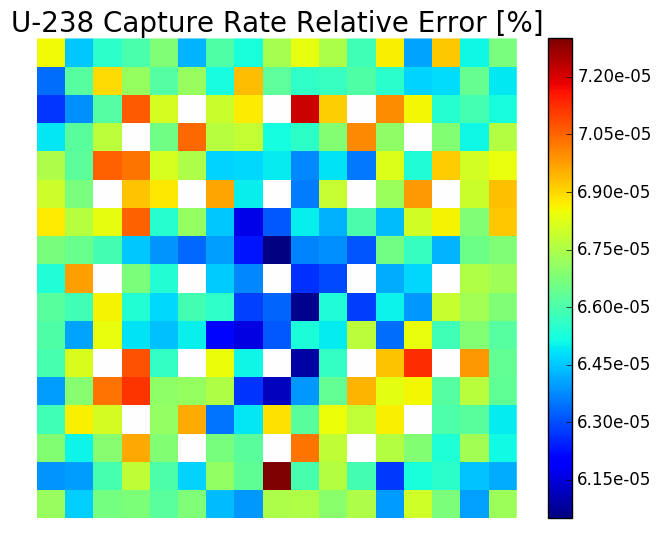
\includegraphics[width=\linewidth]{figures/benchmarks/capture-rates/capt-rel-err-fuel-31-20BAs}
  \caption{}
  \label{fig:chap7-capt-rate-rel-err-3.1-20BAs-assm}
\end{subfigure}%
\caption[U-238 capture rates for a 3.1\% enriched assembly with 20 BPs]{U-238 capture rates for a 3.1\% enriched assembly with 20 \ac{BP}s.}
\label{fig:chap7-capt-rates-3.1-assm-20BAs}
\end{figure}

\begin{figure}[h!]
\centering
\begin{subfigure}{0.5\textwidth}
  \centering
  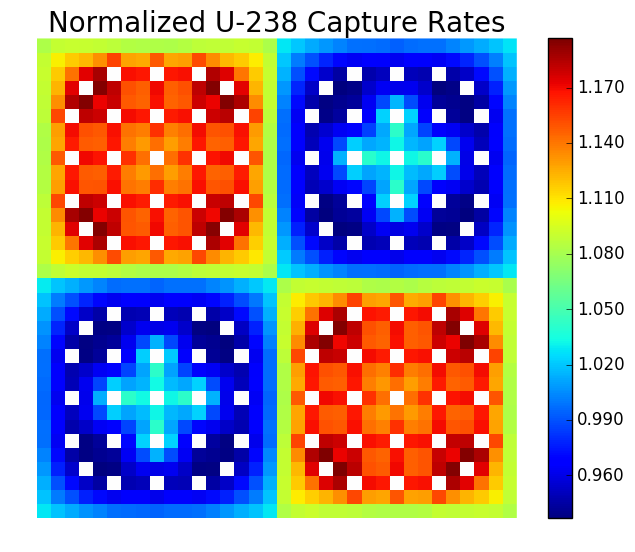
\includegraphics[width=\linewidth]{figures/benchmarks/capture-rates/capt-mean-2x2}
  \caption{}
  \label{fig:chap7-capt-rate-mean-2x2}
\end{subfigure}%
\begin{subfigure}{0.5\textwidth}
  \centering
  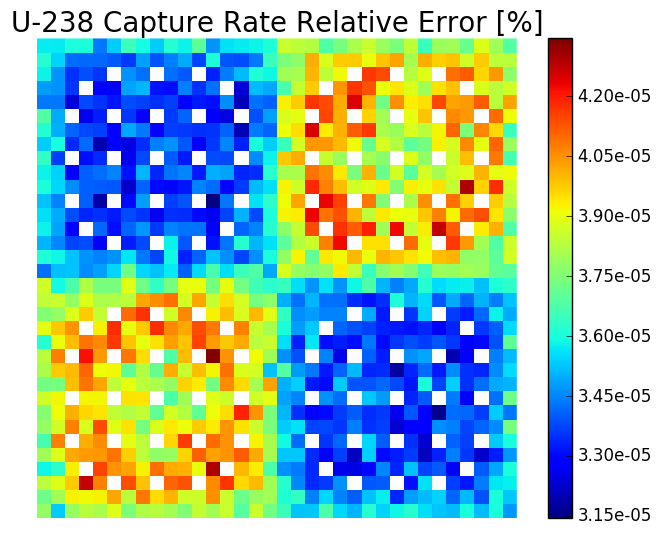
\includegraphics[width=\linewidth]{figures/benchmarks/capture-rates/capt-rel-err-2x2}
  \caption{}
  \label{fig:chap7-capt-rate-rel-err-2x2}
\end{subfigure}%
\caption[U-238 capture rates for a 2$\times$2 colorset]{U-238 capture rates for a 2$\times$2 colorset.}
\label{fig:chap7-capt-rates-2x2}
\end{figure}

\begin{figure}[h!]
\centering
\begin{subfigure}{0.5\textwidth}
  \centering
  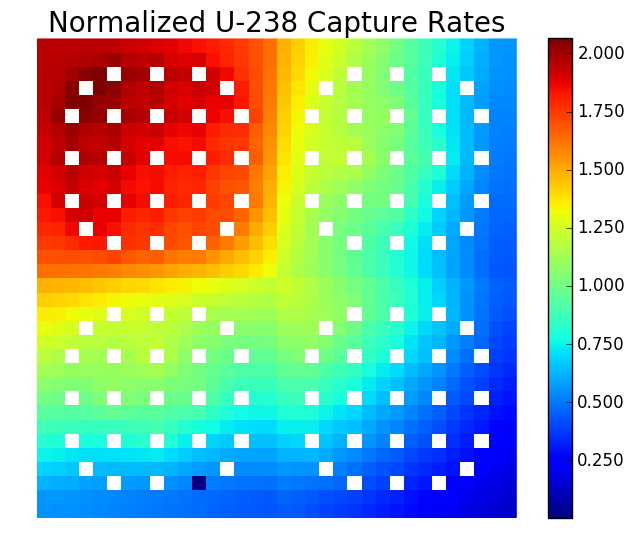
\includegraphics[width=\linewidth]{figures/benchmarks/capture-rates/capt-mean-reflector}
  \caption{}
  \label{fig:chap7-capt-rate-mean-reflector}
\end{subfigure}%
\begin{subfigure}{0.5\textwidth}
  \centering
  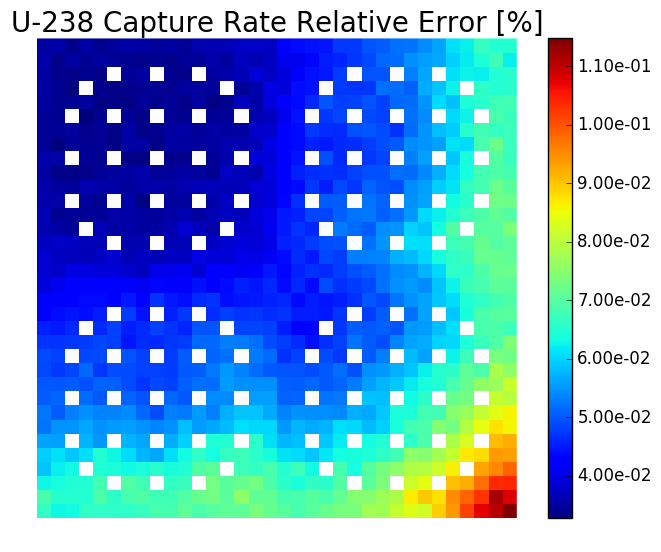
\includegraphics[width=\linewidth]{figures/benchmarks/capture-rates/capt-rel-err-reflector}
  \caption{}
  \label{fig:chap7-capt-rate-rel-err-reflector}
\end{subfigure}%
\caption[U-238 capture rates for a 2$\times$2 colorset with a reflector]{U-238 capture rates for a 2$\times$2 colorset with a reflector.}
\label{fig:chap7-capt-rates-2x2}
\end{figure}

\begin{figure}[h!]
\centering
\begin{subfigure}{0.5\textwidth}
  \centering
  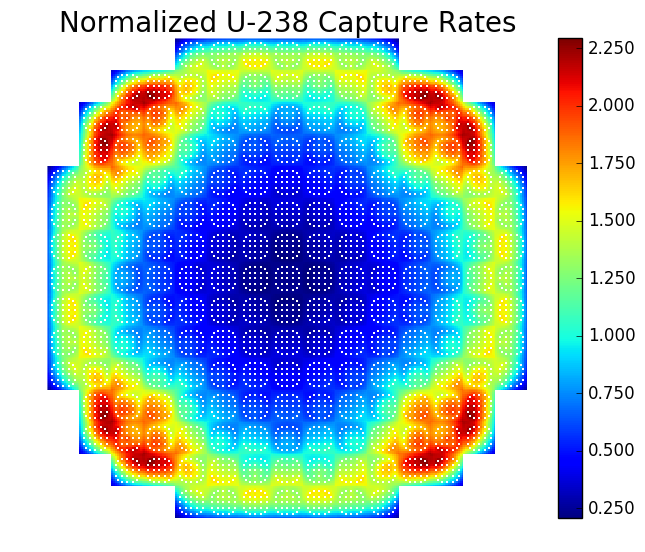
\includegraphics[width=\linewidth]{figures/benchmarks/capture-rates/capt-mean-full-core}
  \caption{}
  \label{fig:chap7-capt-rate-mean-full-core}
\end{subfigure}%
\begin{subfigure}{0.5\textwidth}
  \centering
  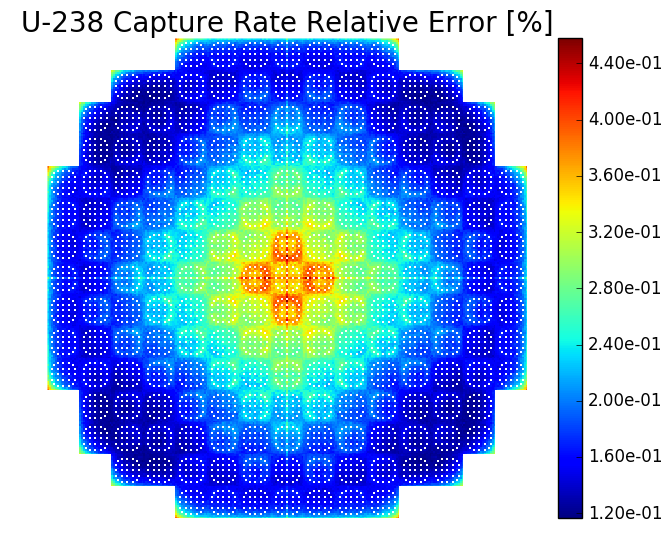
\includegraphics[width=\linewidth]{figures/benchmarks/capture-rates/capt-rel-err-full-core}
  \caption{}
  \label{fig:chap7-capt-rate-rel-err-full-core}
\end{subfigure}%
\caption[U-238 capture rates for the full 2D BEAVRS core]{U-238 capture rates for the full 2D \ac{BEAVRS} core.}
\label{fig:chap7-capt-rates-full-coe}
\end{figure}

\begin{figure}[h!]
\centering
\begin{subfigure}{\textwidth}
  \centering
  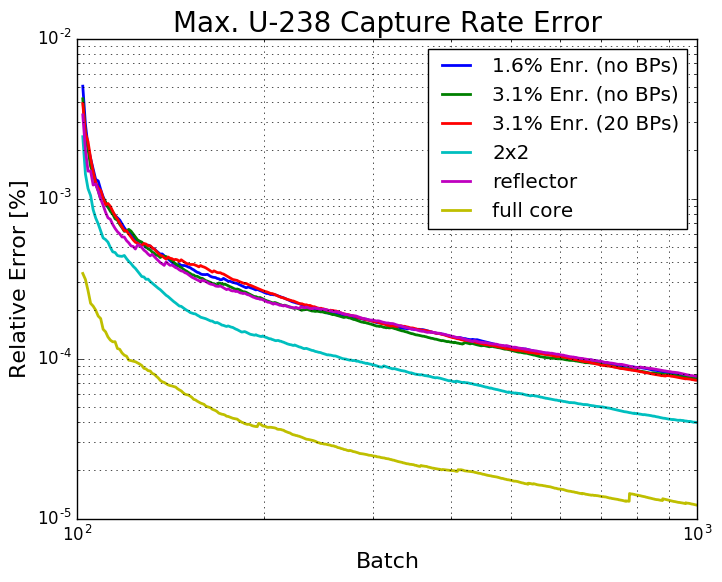
\includegraphics[width=0.8\linewidth]{figures/benchmarks/capture-rates/capt-conv-max-assms}
  \caption{}
  \label{fig:chap7-capt-rate-max-conv}
\end{subfigure}
\begin{subfigure}{\textwidth}
  \centering
  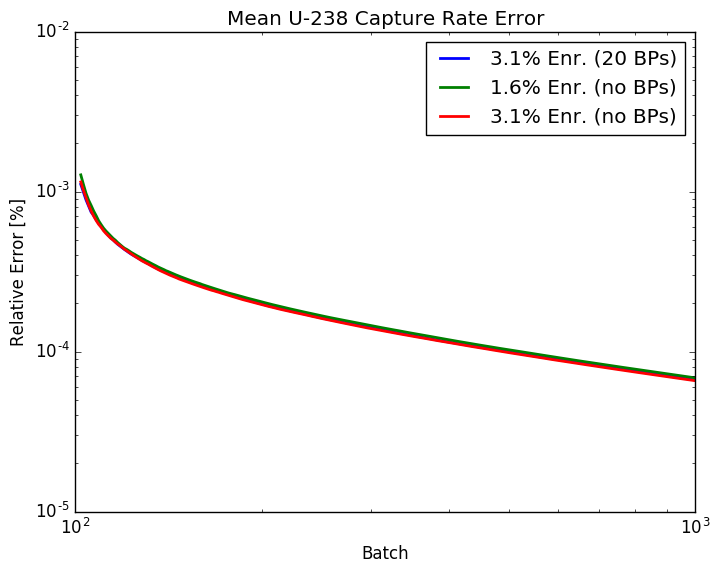
\includegraphics[width=0.8\linewidth]{figures/benchmarks/capture-rates/capt-conv-mean-assms}
  \caption{}
  \label{fig:chap7-capt-rate-max-conv}
\end{subfigure}
\caption[U-238 capture rate error convergence for BEAVRS geometries]{U-238 capture rate relative error convergence for \ac{BEAVRS} fuel geometries.}
\label{fig:chap7-capt-rates-conv}
\end{figure}


-summary box!!!!